This section covers a \gls{VV} study based on the \gls{MSRE} zero-power pump
start-up and coast-down pump transient tests. In collaboration with Aaron Reynolds (formerly from
Oregon State University, we verified and validated the looped \gls{DNP} flow modeling capability of
our respective reactor simulation software, Moltres and QuasiMolto \cite{reynolds_analysis_2023}.

\subsection{Description of MSRE Pump Transient Tests}

The \gls{MSRE} was an experimental molten salt reactor constructed and operated at \gls{ORNL} in
the 1960s \cite{haubenreich_experience_1970}. It is a 8-MW$_{\text{th}}$, thermal-spectrum reactor
with a graphite moderator and a LiF-BeF$_2$-ZrF$_4$-UF$_4$ fuel-molten salt mixture. Under normal
power operation, the fuel salt flows out of the core and deposits heat in the heat exchanger before
being pumped back into the core. Due to
\glspl{DNP} being produced in the molten salt coolant, flow rates have significant impacts on the
\gls{DNP} distribution and reactivity. Delayed neutrons born in regions of lower neutronic
importance, e.g., at the periphery or outside the core, are more likely to be lost through neutron
leakage or parasitic absorption.

\begin{figure}[htb]
  \centering
  \begin{minipage}[t]{0.49\textwidth}
    \centering
    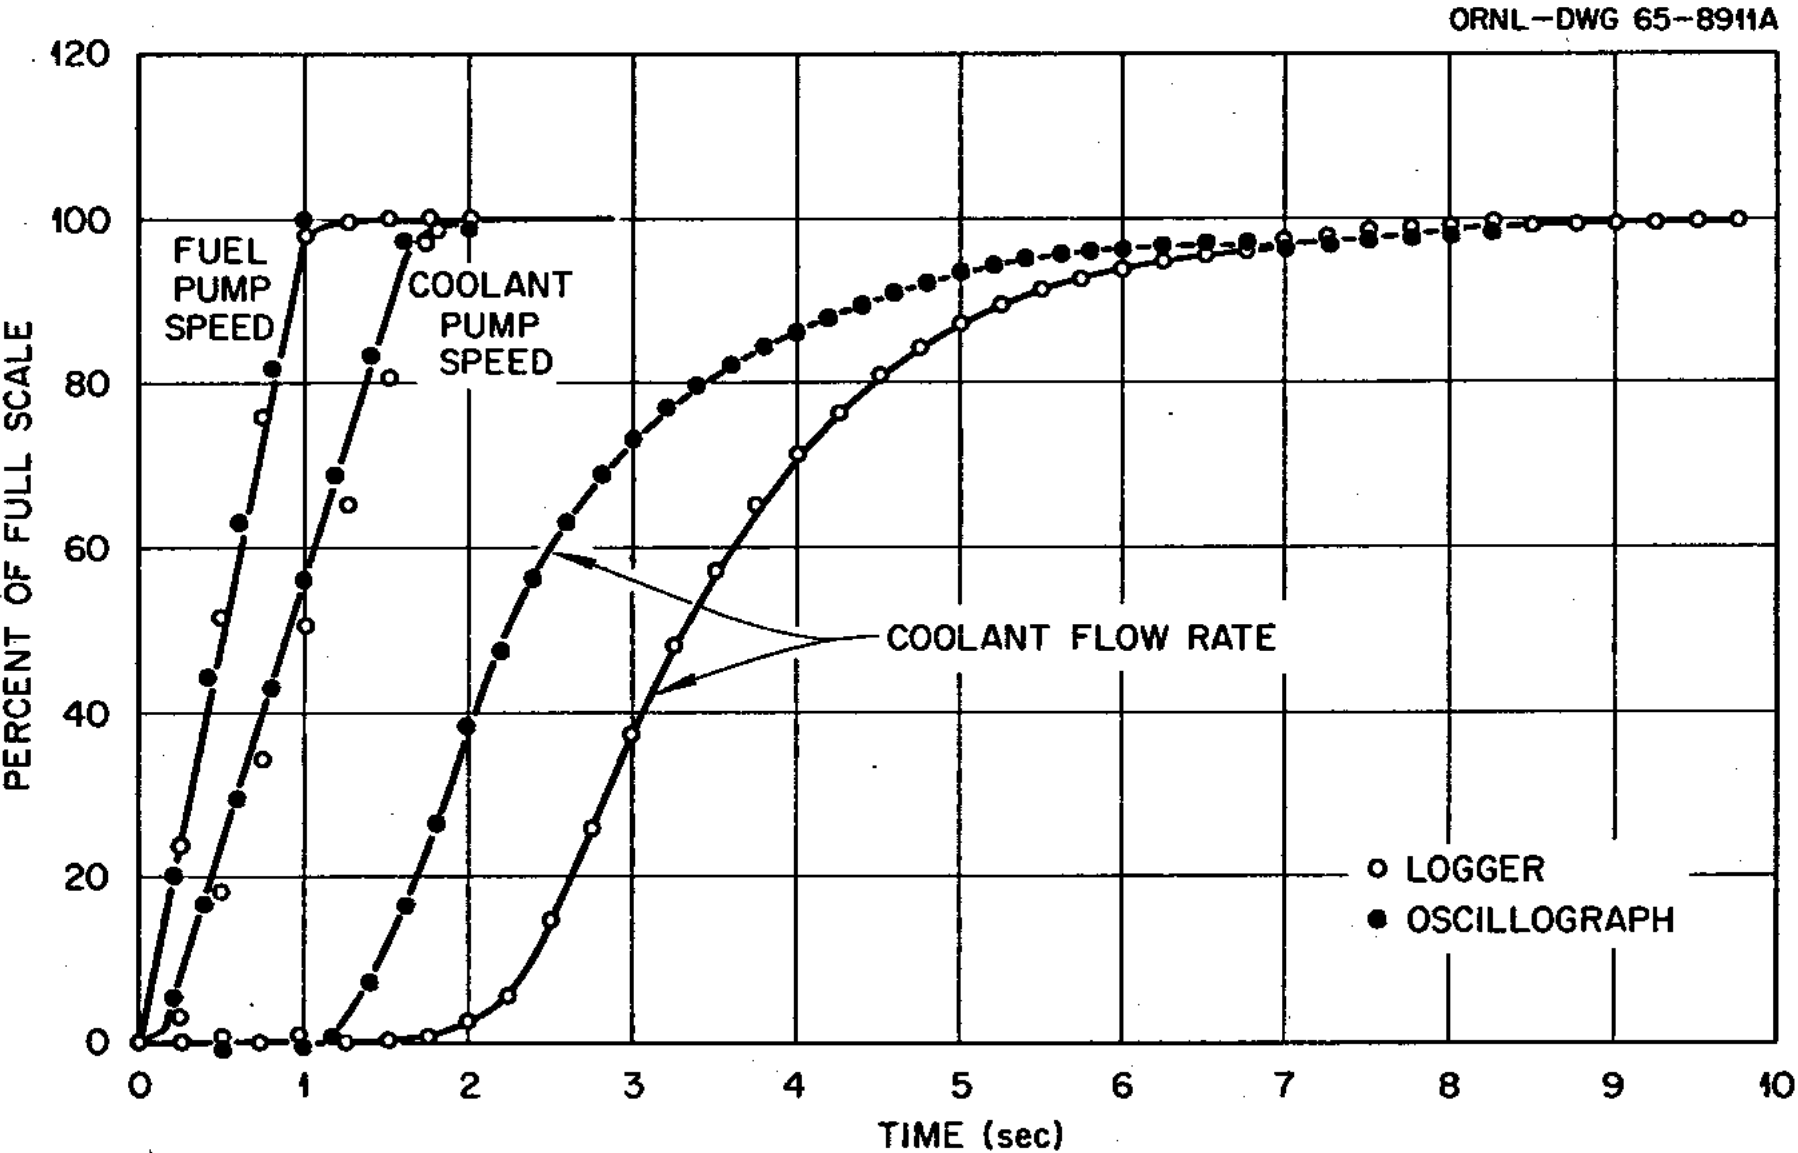
\includegraphics[width=\columnwidth]{msre-startup}
    \caption{Start-up pump speed and coolant flow rate \cite{prince_zero-power_1968}.}
    \label{fig:msre-startup}
  \end{minipage}
  \hfill
  \begin{minipage}[t]{0.49\textwidth}
    \centering
    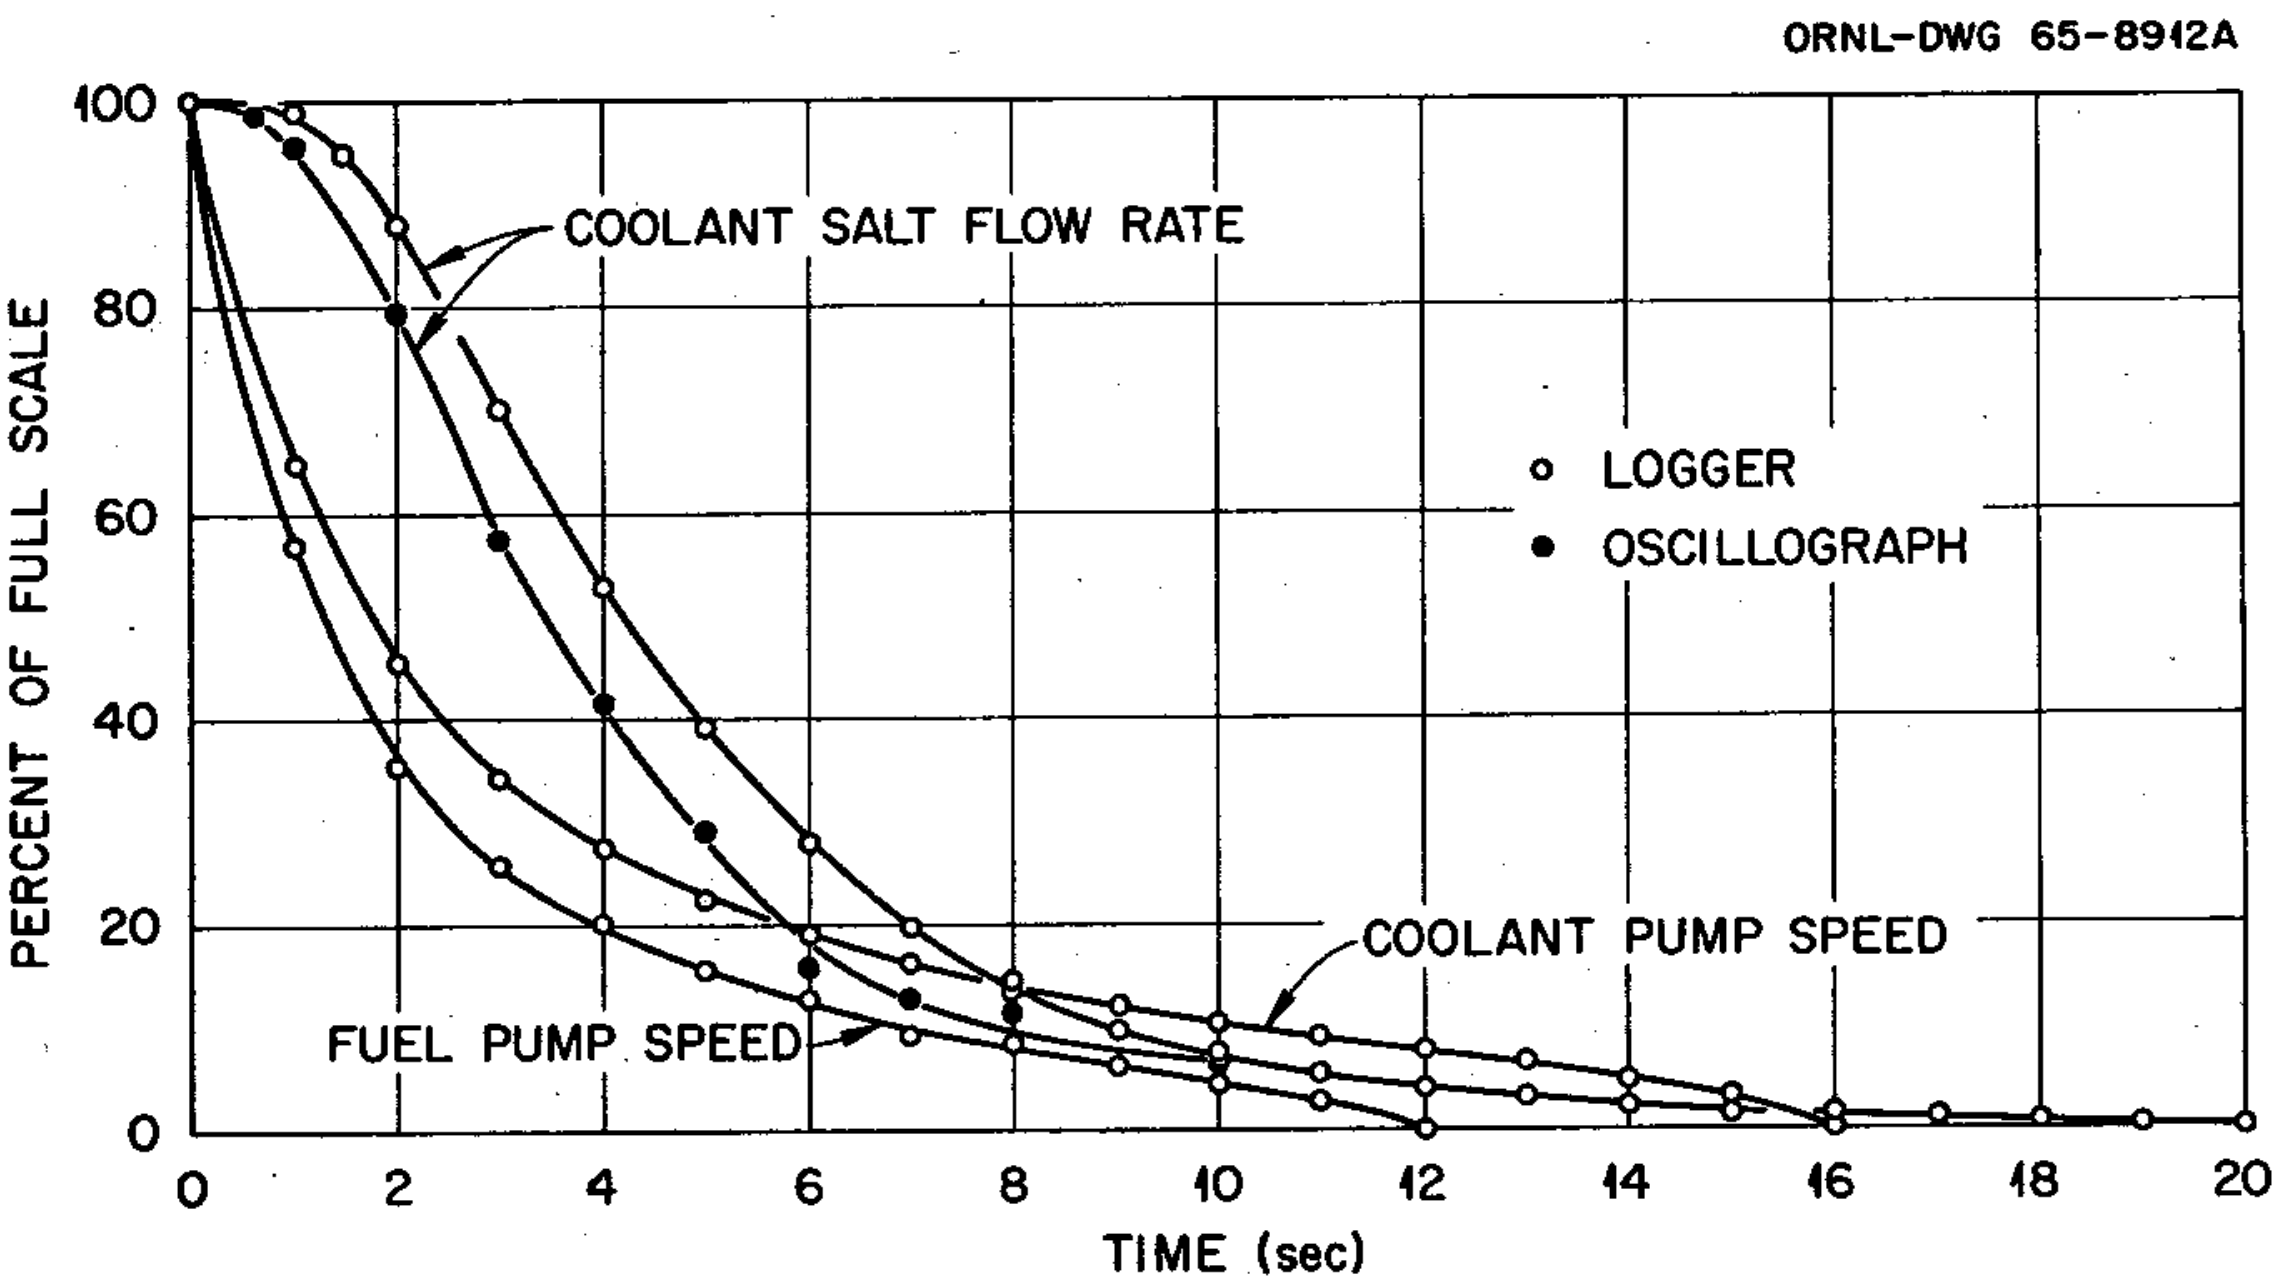
\includegraphics[width=\columnwidth]{msre-coastdown}
    \caption{Coast-down pump speed and coolant flow rate \cite{prince_zero-power_1968}.}
    \label{fig:msre-coastdown}
  \end{minipage}
\end{figure}

\gls{ORNL} researchers performed fuel pump start-up and coast-down transient experiments to
determine the ``transient effects of fuel flow-rate changes on reactivity''
\cite{prince_zero-power_1968}. These experiments were a part of \gls{MSRE} zero-power dynamics
tests performed in June 1965, the same month the \gls{MSRE} achieved initial criticality. Figures
\ref{fig:msre-startup} and \ref{fig:msre-coastdown} show the pump speeds and secondary salt coolant
flow rates measured during the transients. The changing flow rates caused advective changes to the
\gls{DNP} distribution and the \gls{DNF} in the reactor core.

During both experiments, the reactivity effects of the \gls{DNP} drift were measured by
allowing the flux servo controller to maintain criticality. The controller maintained core
criticality by adjusting the control rod insertion height in response to \gls{DNP} drift-induced
reactivity changes. The reactivity changes over time can be calculated by comparing the various
control rod positions (Figure \ref{fig:msre-pump-rod}) with the control rod integral worth curve
(Figure \ref{fig:msre-rod-worth}) obtained during control rod calibration experiments.

\begin{figure}[htb]
  \centering
  \begin{minipage}[t]{0.49\textwidth}
    \centering
    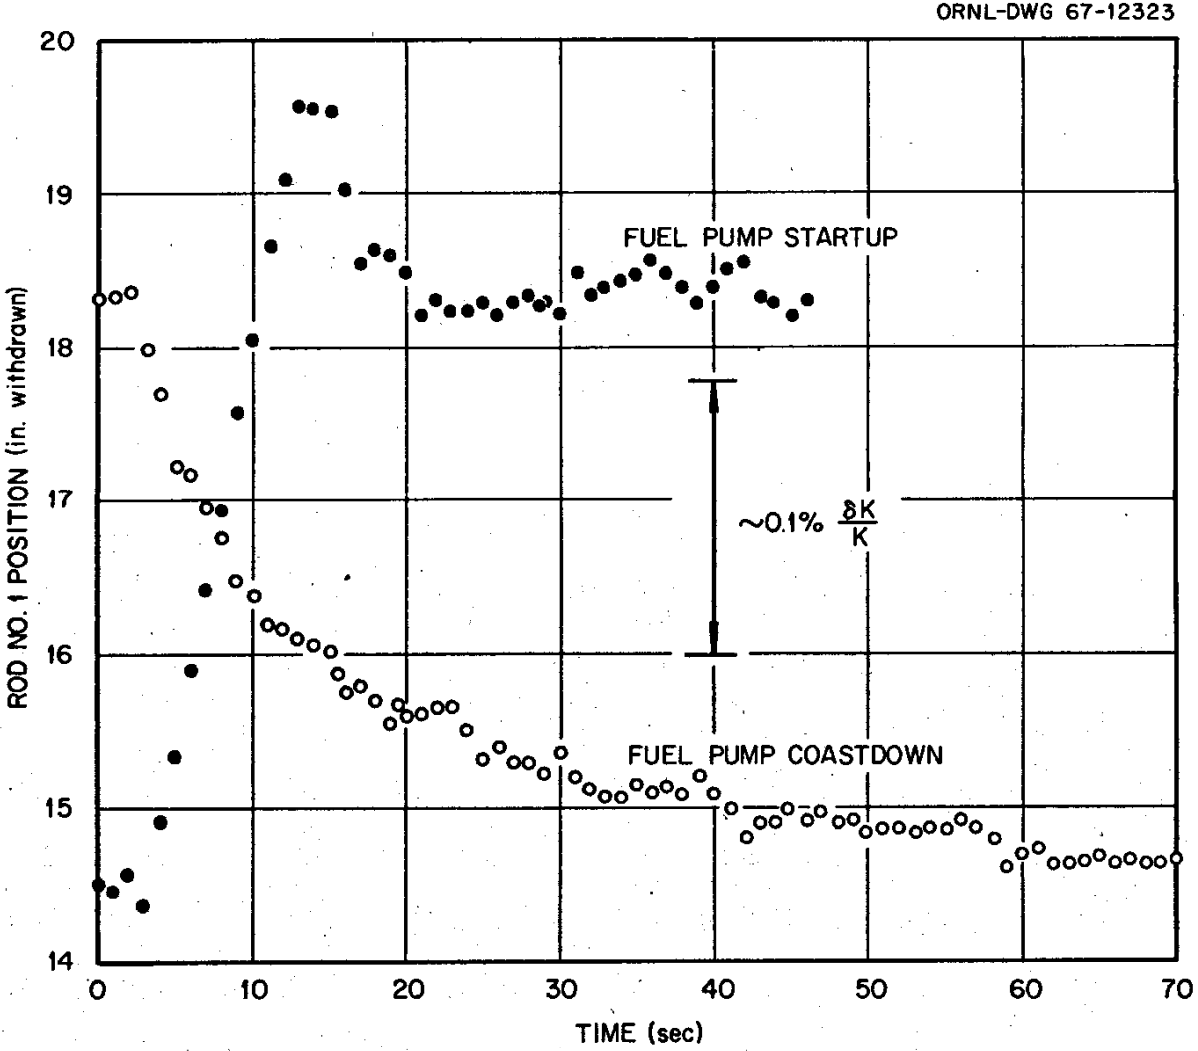
\includegraphics[width=\columnwidth]{msre-transient}
    \caption{Control rod response to fuel pump start-up and coast-down
    \cite{prince_zero-power_1968}.}
    \label{fig:msre-pump-rod}
  \end{minipage}
  \hfill
  \begin{minipage}[t]{0.49\textwidth}
    \centering
    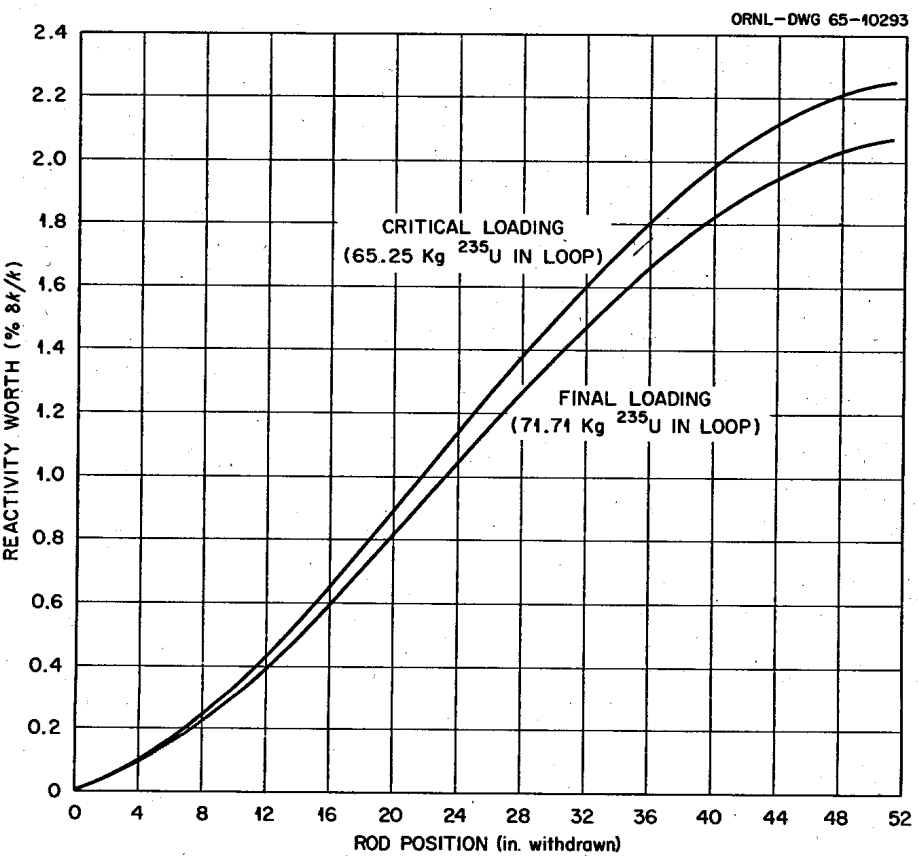
\includegraphics[width=\columnwidth]{msre-rod-worth}
    \caption{Integral control rod worth of Rod 1 \cite{prince_zero-power_1968}.}
    \label{fig:msre-rod-worth}
  \end{minipage}
\end{figure}

\subsection{Description of QuasiMolto}

QuasiMolto \cite{reynolds_analysis_2023} is an open-source multiphysics research code for
simulating circulating fuel reactor kinetics. It uses the multilevel \gls{QD} methodology described
in Section \ref{sec:lit-tc} to model multigroup neutron transport with \gls{DNP} flow and
temperature advection-diffusion. Consisting of three levels of neutron calculations, the highest
level solves the multigroup high-order transport equations for Eddington and boundary factors which
populate previously unknown quantities in the mid-level multigroup low-order \gls{QD} equations.
In turn, the mid-level equations solve for group-collapsed Eddington and boundary factors for the
low-level effective low-order transport equations. The effective low-order transport equations
couple with the \gls{DNP} and temperature governing equations for multiphysics reactivity feedback
from temperature and \gls{DNP} flow. Readers may refer to the linked reference
\cite{reynolds_analysis_2023} for more details on QuasiMolto.

QuasiMolto applies the simple corner balance method
\cite{adams_subcell_1997} for spatial discretization.
For this study, the QuasiMolto \gls{MSRE} model employed $S_2$ neutron transport to facilitate
fair comparisons with the neutron diffusion method in Moltres. For time-dependent \gls{DNP} flow
modeling, QuasiMolto applies implicit Euler scheme for the reaction
and diffusion terms, and explicit Superbee flux limiter scheme for the advection term.

\subsection{Modeling Approach}

For this study, we adopted a 2-D axisymmetric (R-Z) model of the \gls{MSRE} consisting of
alternating vertical regions of molten salt and graphite moderator. This is the same \gls{MSRE}
model Reynolds developed for his PhD thesis \cite{reynolds_multilevel_2020} and a related
journal publication \cite{reynolds_analysis_2023}. Figure \ref{fig:pump-geom} depicts the 2-D
axisymmetric \gls{MSRE} model. The fuel salt channels are 1.25-cm wide and spaced at 5-cm intervals
in the graphite matrix. The fuel salt volume fraction of this model is 0.236, differing
slightly to the \gls{MSRE} design specification of 0.225 \cite{robertson_msre_1965}. The geometry
mesh is uniform with a width of $\Delta r=0.078125$ cm and height of $\Delta z=5$ cm.
Vacuum boundary conditions for the neutron flux apply along the top, bottom, and right boundaries.

The salt flows
upwards at a spatially uniform velocity rate of 18.085 cm s$^{-1}$. \glspl{DNP} flow out of the
core model and through a separate 285-cm long 1-D pipe model before being reintroduced through the
bottom core channel inlets. The 1-D pipe length maintains the overall salt circulation time of
25.2 s from the \gls{MSRE} design specification \cite{robertson_msre_1965}. Note that the salt
velocity and 1-D pipe length in this study differs from the \gls{MSRE} model described in Reynolds'
paper \cite{reynolds_analysis_2023}. We reduced the velocity to compensate for the absence of upper
and lower core plena by extending salt residence time in the salt-graphite lattice region.

\begin{figure}[htb]
  \centering
  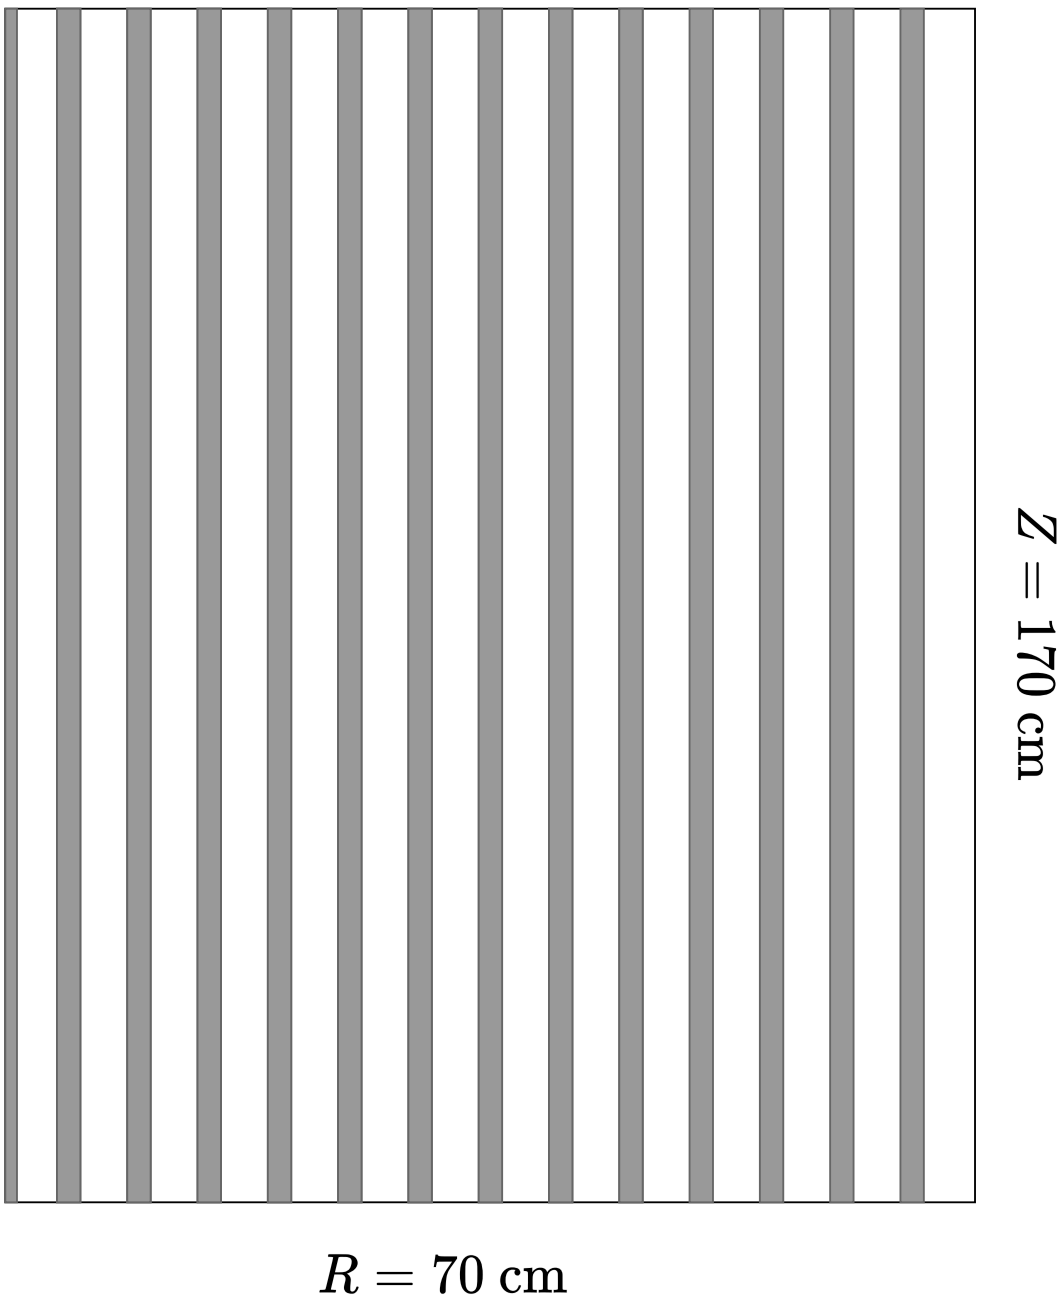
\includegraphics[width=0.6\columnwidth]{msre-2d}
  \caption{2-D axisymmetric model of the \gls{MSRE}.The gray and white regions represent fuel salt
  and graphite, respectively. The leftmost fuel salt channel falls along the axis of symmetry and
  is half-width. Not drawn to scale.}
  \label{fig:pump-geom}
\end{figure}

Reynolds generated group constants for two neutron energy groups and six \gls{DNP} groups using the
NEWT transport module within the SCALE code system \cite{rearden_scale_2018} and the ENDF/B-VII
nuclear data library \cite{chadwick_endf/b-vii.1_2011}. The SCALE model geometry comprised a
representative unit cell geometry
consisting of a circular fuel region in the center of a square graphite region and reflective
boundary conditions on all boundaries. The unit cell dimensions preserved material compositions
and salt-to-graphite ratios from the \gls{MSRE} design specifications.

Prior to the pump transient simulations, we performed code-to-code verification by comparing the
$k_\text{eff}$ and neutron flux and \gls{DNP} distributions of the 2-D \gls{MSRE} model under
static, no salt flow conditions. We sampled the neutron flux and \gls{DNP} distributions on
mesh corners and edge centers along the centerline ($r=0$ cm) and midplane ($z=85$ cm) of the
reactor geometry.

In lieu of reactivity control using a control rod in the pump
transient simulations, QuasiMolto and Moltres solved their respective
two-group $k$-eigenvalue neutronics models at every time-step. The $1/k_\text{eff}$ scaling factor
in the fission neutron source term keeps the simulation at a pseudo-critical state. The \gls{DNP}
source term is also scaled by $1/k_\text{eff}$ at every time-step. We interpolated the \gls{MSRE}
salt flow velocity data in Figures \ref{fig:msre-startup} and \ref{fig:msre-coastdown} to apply in
our pump start-up and coast-down simulations. The pump start-up simulation starts from a static
state with no salt flow while the pump coast-down simulation starts from a steady flow state with
operating salt flow.

\subsection{Results \& Discussion}

We start with a comparison of the Moltres and QuasiMolto \gls{MSRE} numerical models under static
and steady salt flow conditions. Table \ref{table:msre-pump-keff} lists the $k_\text{eff}$
estimates under static and steady flow conditions, and the reactivity changes due to \gls{DNP}
flow. Moltres and QuasiMolto show excellent agreement with 22 and 21 pcm absolute differences in
$k_\text{eff}$ under static and steady flow conditions, respectively. Consequently, the
$\Delta\rho$ estimates from \gls{DNP} flow fall within 1 pcm difference of each other.

\begin{table}[htb]
  \centering
  \caption{Multiplication factors $k_\text{eff}$ under static and steady salt flow conditions, and
  reactivity changes $\Delta\rho$ due to \gls{DNP} flow from the Moltres and QuasiMolto \gls{MSRE}
  models.}
  \begin{tabular}{l S S S}
    \toprule
    \multirow{2}{*}{Code} & \multicolumn{2}{c}{$k_\text{eff}$} & {$\Delta\rho$ due to} \\
                          & {Static} & {Steady flow} & {\gls{DNP} flow} \\
                          \cmidrule(r){1-1} \cmidrule(rl){2-3} \cmidrule(l){4-4}
    Moltres & 1.05625 & 1.05311 & -282.4 \\
    QuasiMolto & 1.05603 & 1.05290 & -281.7 \\
    \bottomrule
  \end{tabular}
  \label{table:msre-pump-keff}
\end{table}

Moving on to comparing spatial distributions, we start with the centerline neutron flux
distributions. Figure \ref{fig:centerline-flux-dist} shows the normalized group 1 and 2 neutron
fluxes exhibiting nearly perfect overlap. The flux ratio distributions in Figure
\ref{fig:centerline-flux-ratio} illustrate the strong agreement between Moltres and QuasiMolto at
all sampled locations with the relative differences falling below 0.8\%. We attribute
the oscillations in the flux ratios to differences in spatial discretization schemes. Moltres
uses \gls{FEM} with 1st-order flux values computed at the mesh corners. QuasiMolto uses
the simple corner balance method which subdivides each mesh element into four equal subcells and
computes volume-averaged flux values in each subcell. As such, Moltres and QuasiMolto require
interpolation for sampling mesh edge center and mesh corner values, respectively. The flux ratios
sampled at the top and bottom boundaries show the greatest differences of up to 0.8\%. We attribute
these differences at the boundaries to differences in neutronics methods. The neutron diffusion
method vacuum boundary condition in Moltres depends on the scalar flux gradient (1-st
order derivative) while the $S_2$ method vacuum boundary condition in QuasiMolto depends on the
angular flux value. Combined with the different spatial discretization schemes, flux differences at
the boundary are expected in numerical calculations. Nevertheless, the overall ratio magnitudes
remain small, thereby supporting code-to-code consistency between Moltres and QuasiMolto.

\begin{figure}[htb]
  \centering
  \begin{subfigure}[b]{0.48\columnwidth}
    \centering
    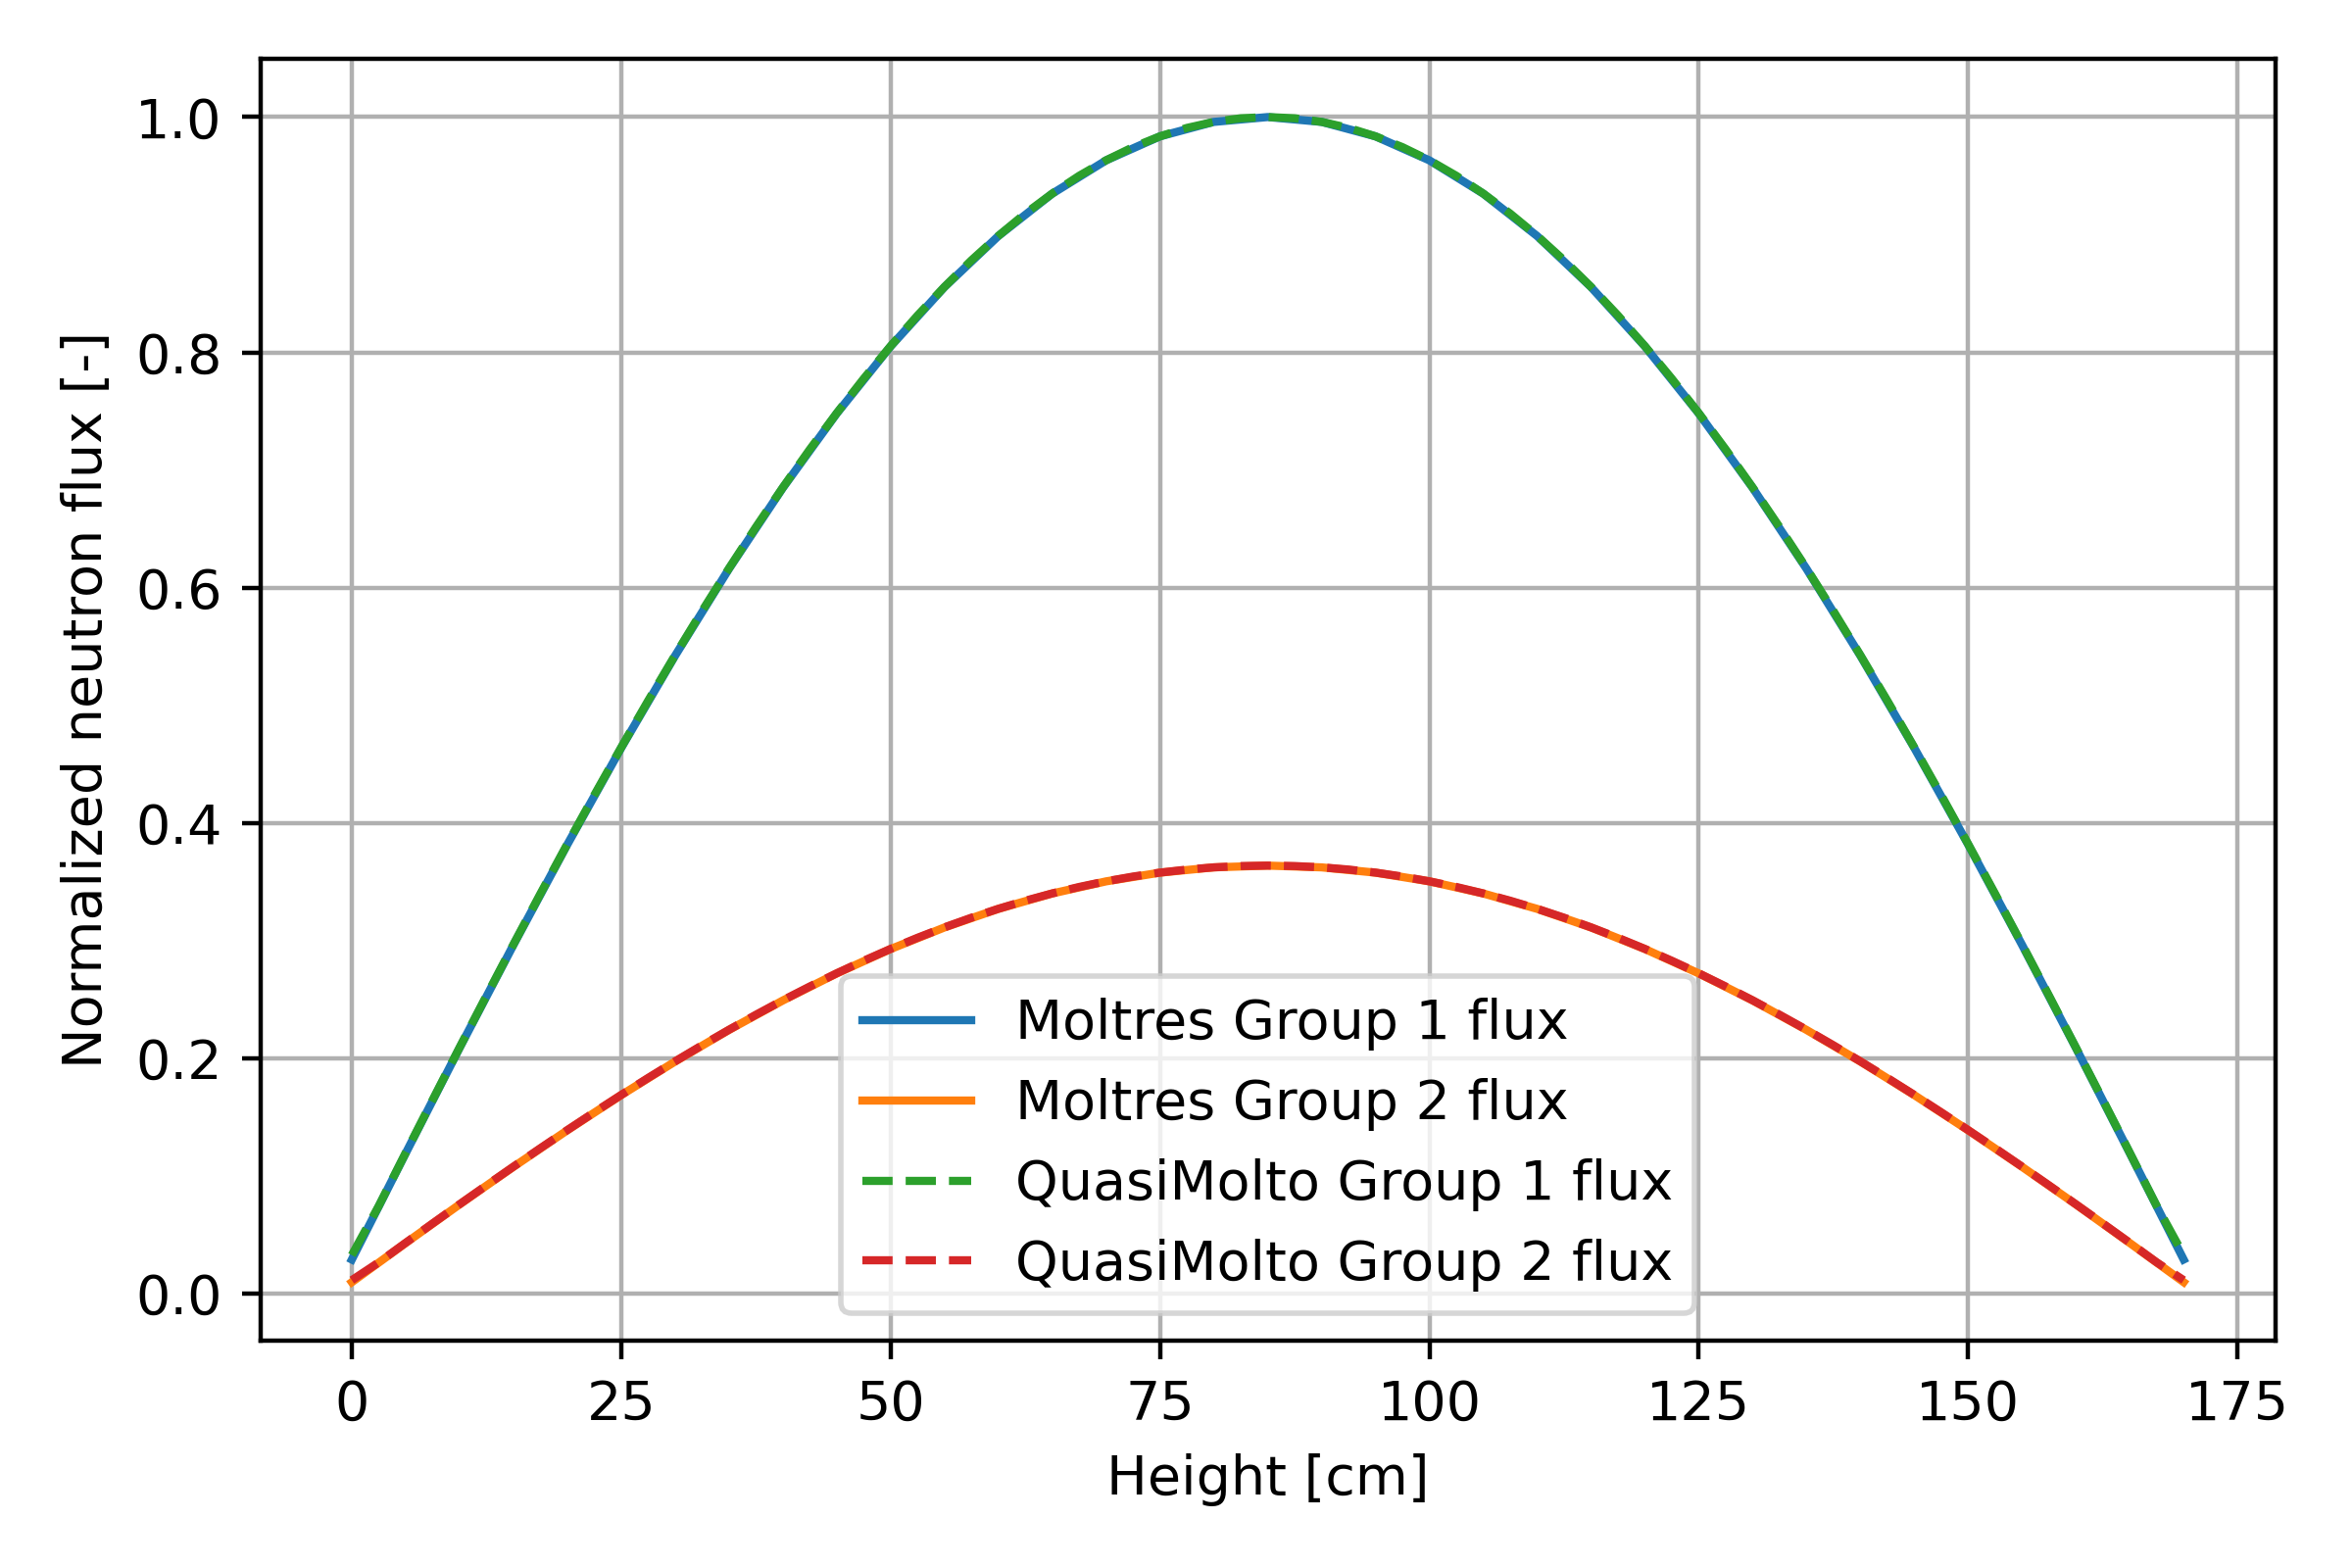
\includegraphics[width=\columnwidth]{centerline_flux}
    \caption{Normalized centerline neutron fluxes.}
    \label{fig:centerline-flux-dist}
  \end{subfigure}
  \hfill
  \begin{subfigure}[b]{0.48\columnwidth}
    \centering
    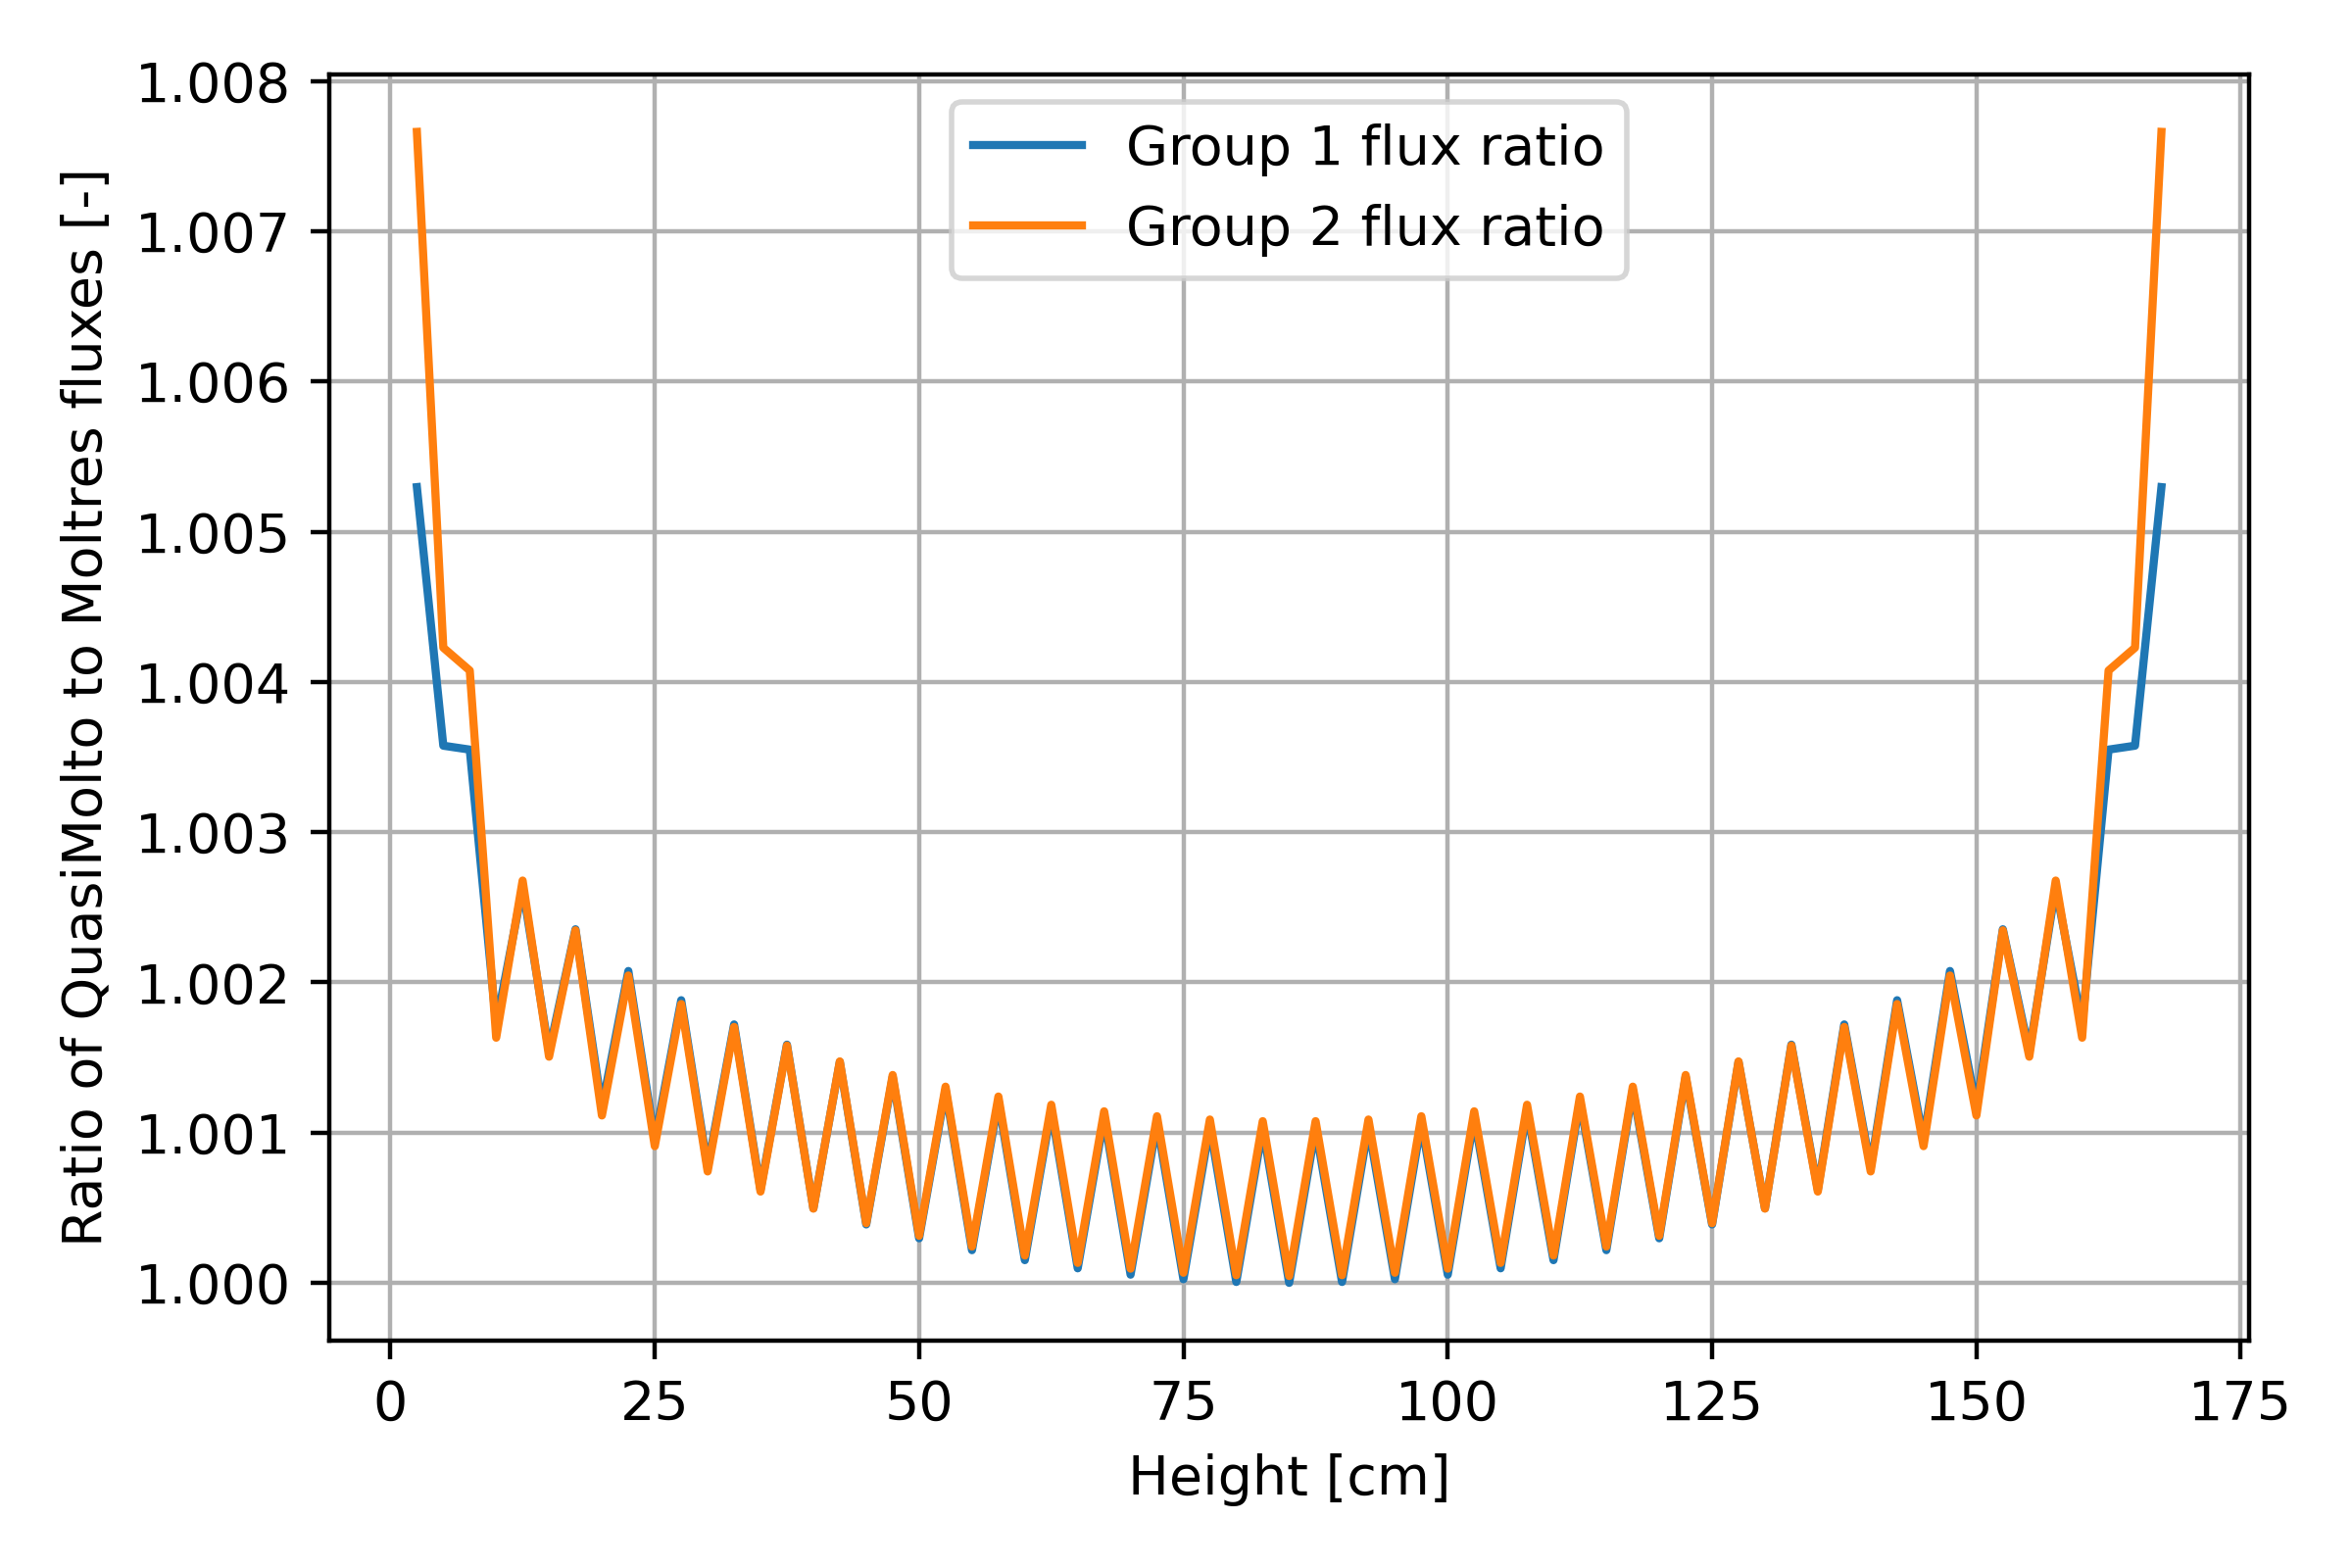
\includegraphics[width=\columnwidth]{centerline_flux_ratio}
    \caption{Ratio of centerline neutron fluxes.}
    \label{fig:centerline-flux-ratio}
  \end{subfigure}
  \caption{Centerline neutron flux distributions and ratios comparing QuasiMolto and Moltres
  \gls{MSRE} models under static conditions.}
  \label{fig:centerline-flux}
\end{figure}

\begin{figure}[htb]
  \centering
  \begin{subfigure}[b]{0.48\columnwidth}
    \centering
    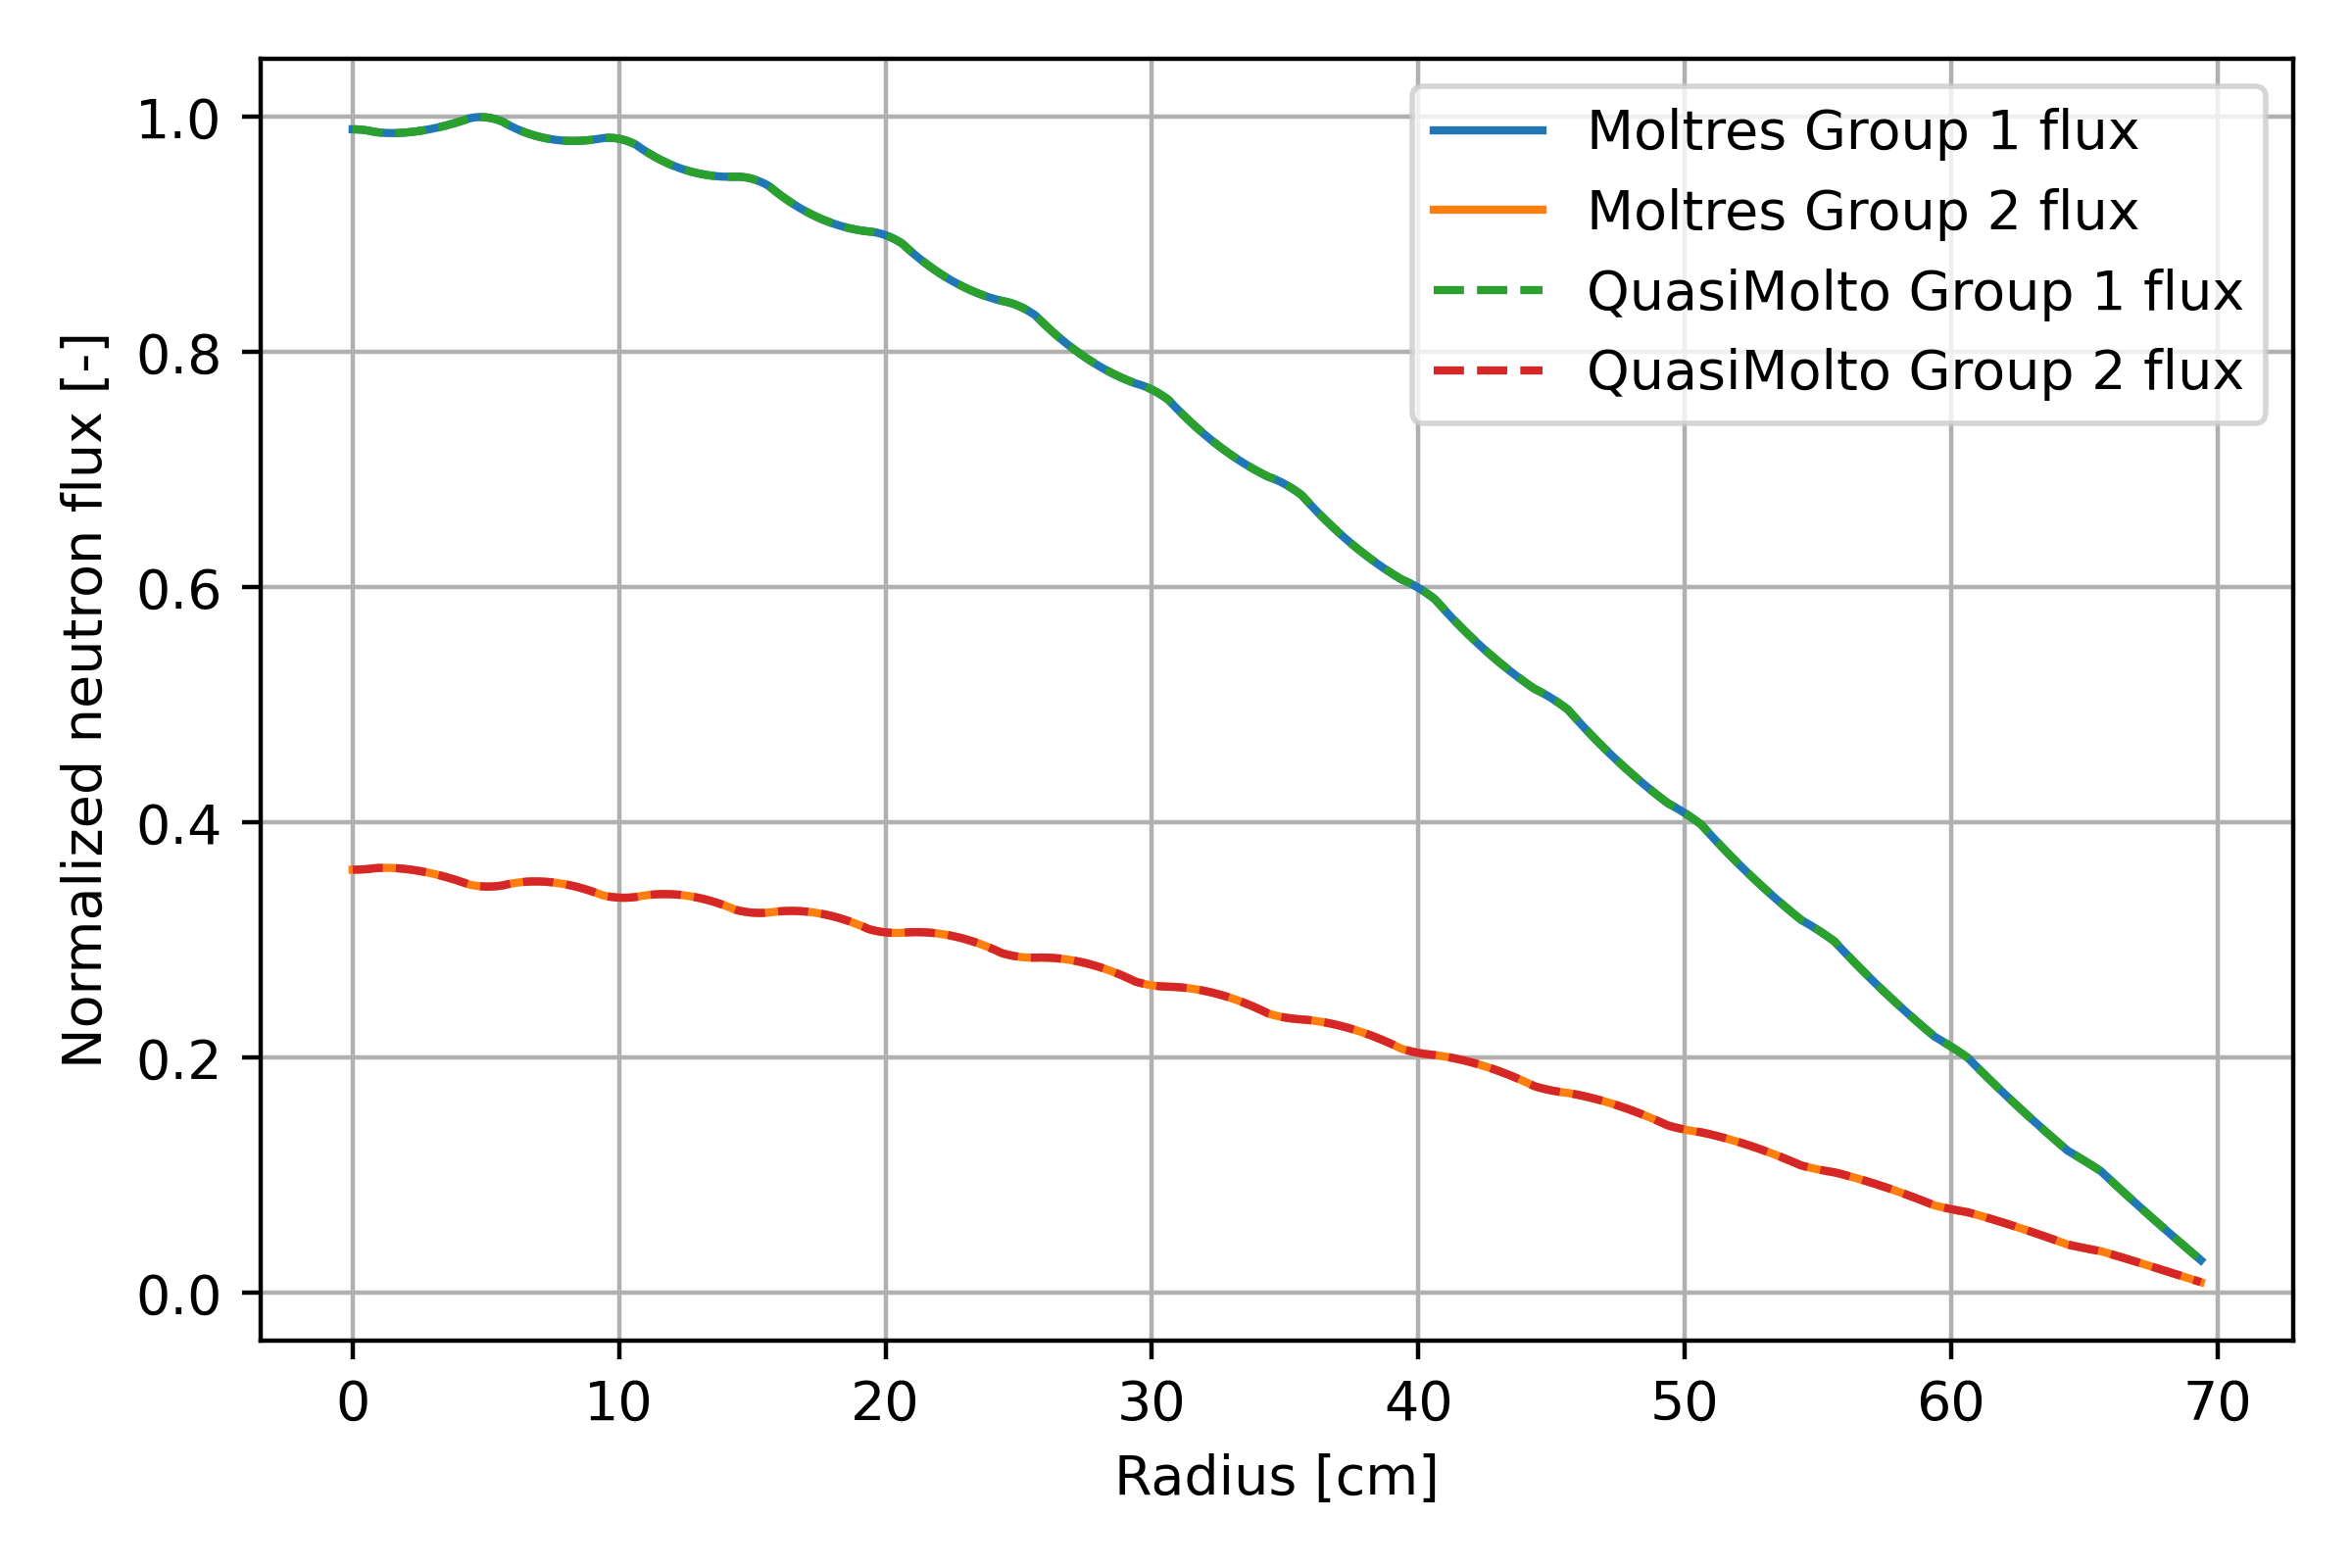
\includegraphics[width=\columnwidth]{midplane_flux}
    \caption{Normalized midplane neutron fluxes.}
    \label{fig:centerline-flux-dist}
  \end{subfigure}
  \hfill
  \begin{subfigure}[b]{0.48\columnwidth}
    \centering
    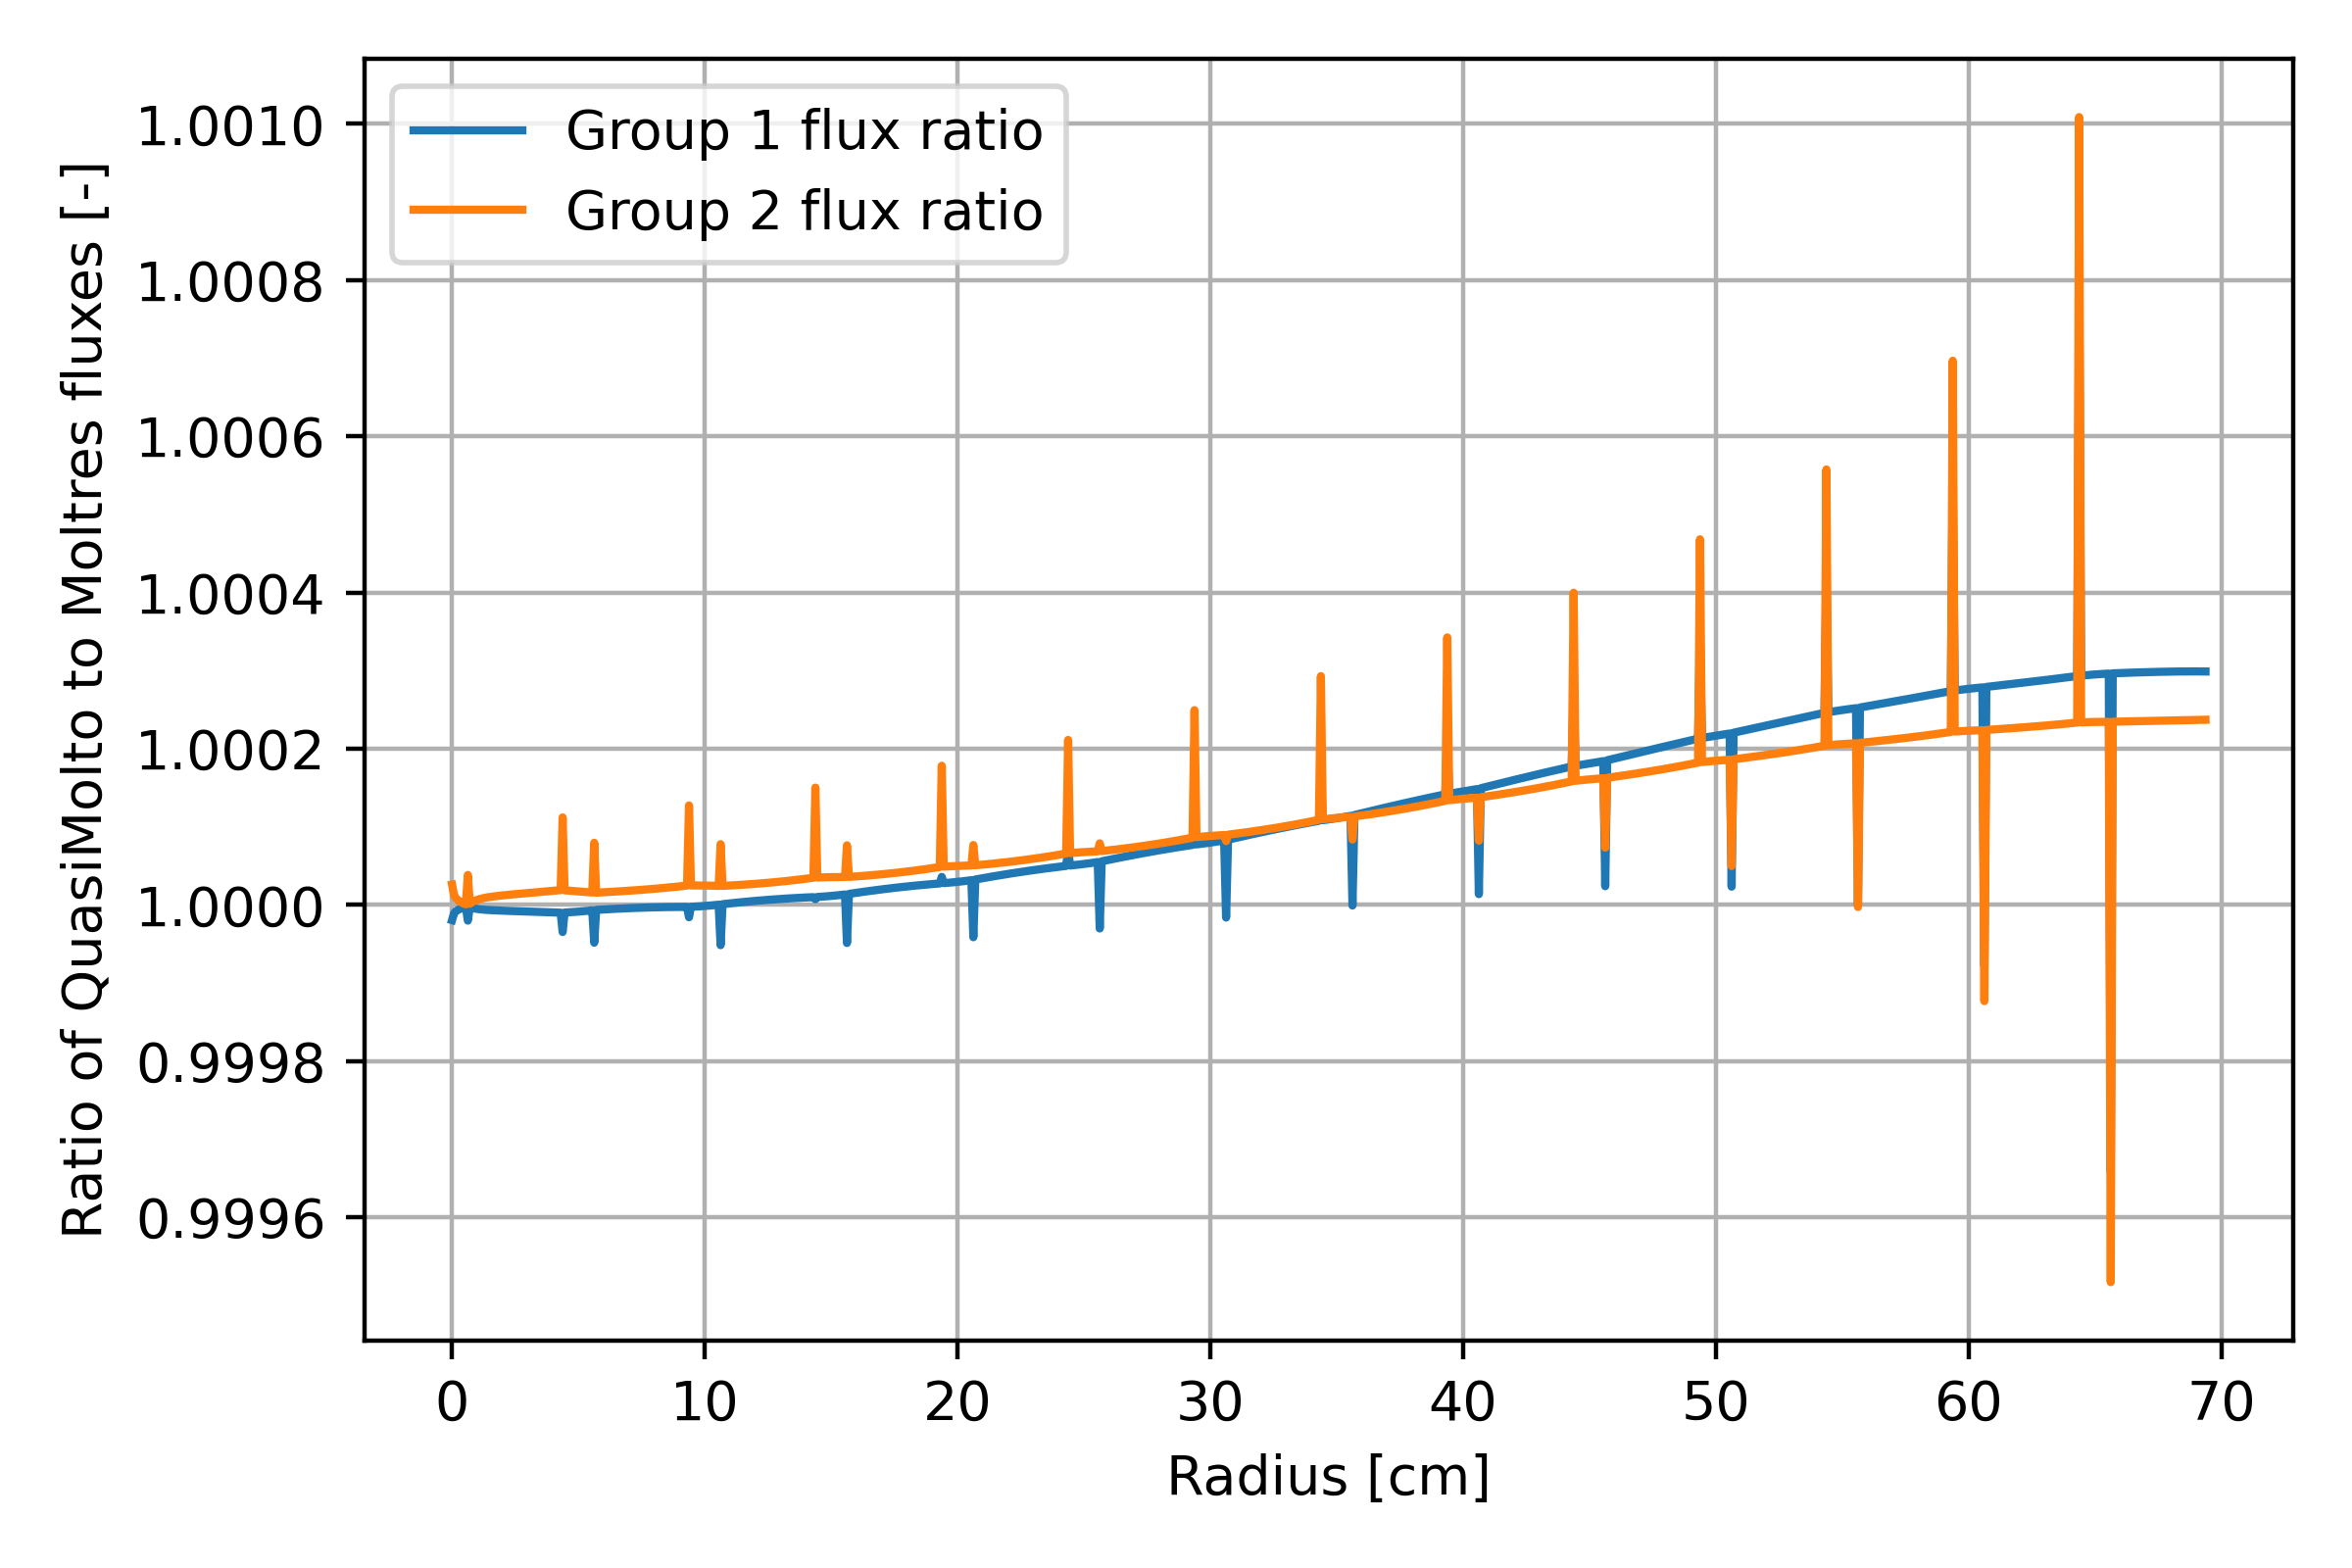
\includegraphics[width=\columnwidth]{midplane_flux_ratio}
    \caption{Ratio of midplane neutron fluxes.}
    \label{fig:centerline-flux-ratio}
  \end{subfigure}
  \caption{Midplane neutron flux distributions and ratios comparing QuasiMolto and Moltres
  \gls{MSRE} models under static conditions.}
  \label{fig:centerline-flux}
\end{figure}

\begin{figure}[htb]
  \centering
  \begin{subfigure}[b]{0.48\columnwidth}
    \centering
    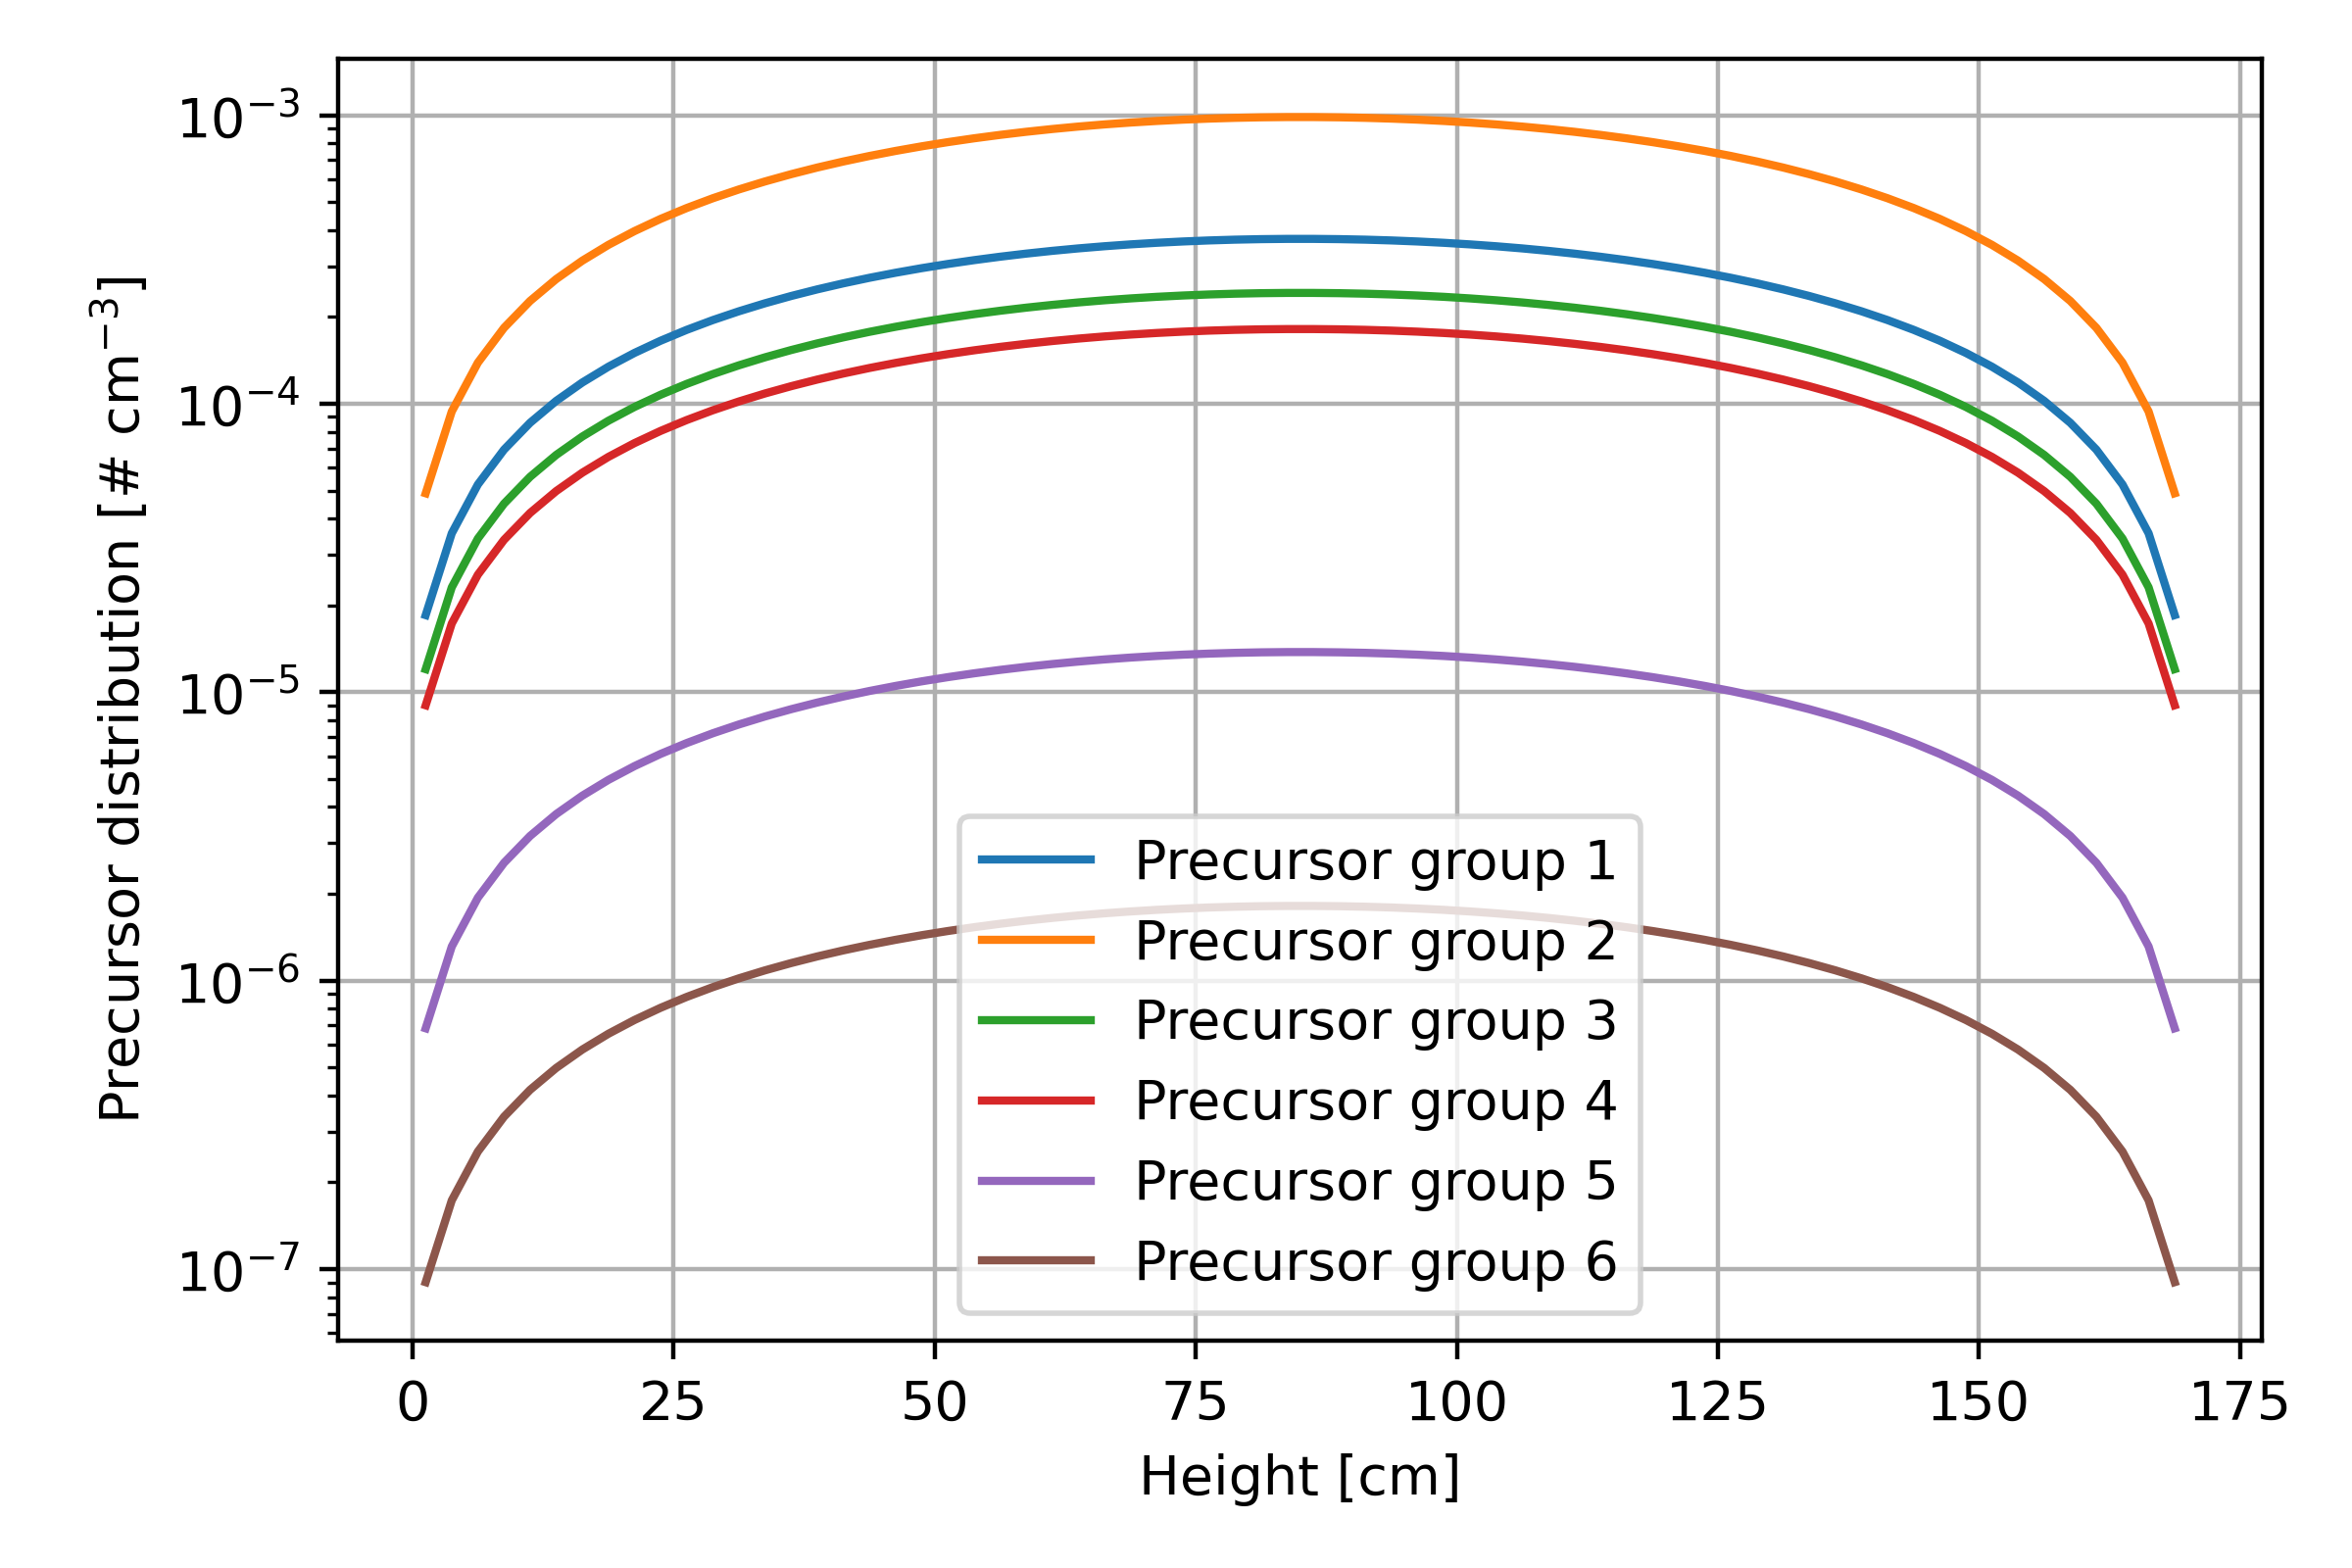
\includegraphics[width=\columnwidth]{centerline_pre}
    \caption{Normalized centerline \gls{DNP} distributions.}
    \label{fig:centerline-pre-dist}
  \end{subfigure}
  \hfill
  \begin{subfigure}[b]{0.48\columnwidth}
    \centering
    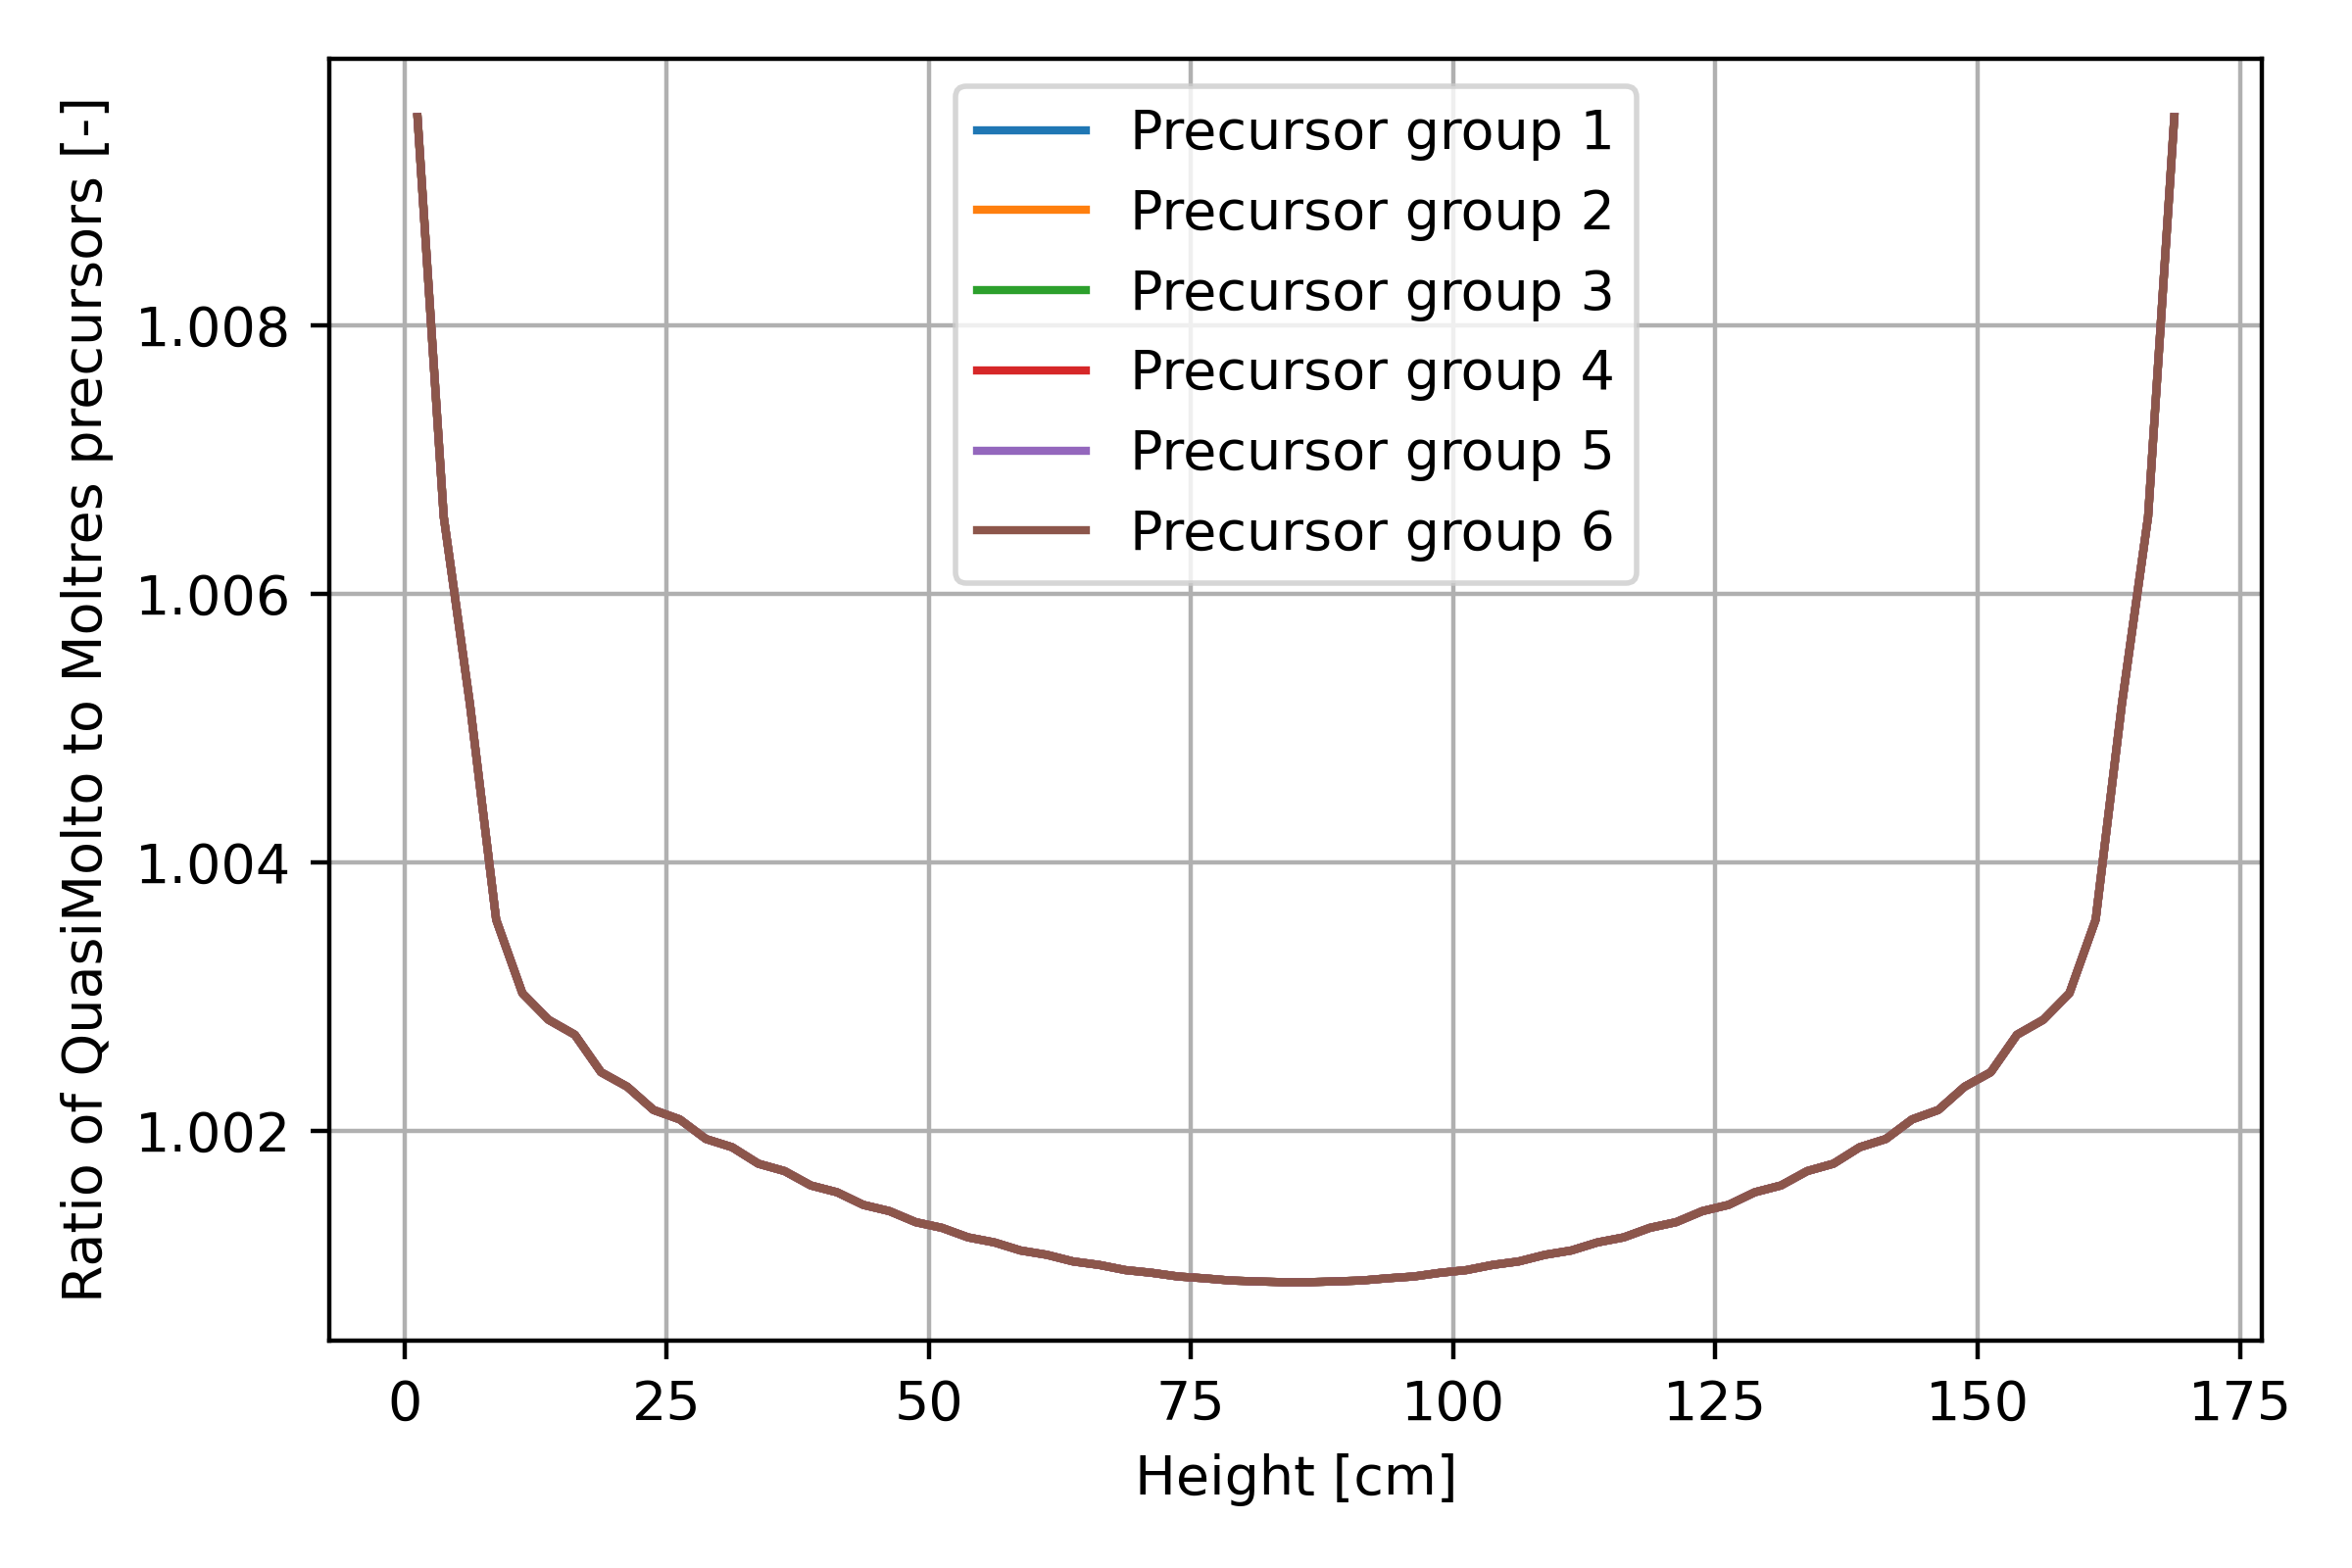
\includegraphics[width=\columnwidth]{centerline_pre_ratio}
    \caption{Ratio of centerline \gls{DNP} distributions.}
    \label{fig:centerline-pre-ratio}
  \end{subfigure}
  \caption{Centerline \gls{DNP} distribution from Moltres and ratios comparing QuasiMolto and
  Moltres models under static \gls{MSRE} conditions. The ratio curves for every \gls{DNP} group
  exhibit nearly perfect overlap.}
  \label{fig:centerline-pre}
\end{figure}

\begin{figure}[htb]
  \centering
  \begin{subfigure}[b]{0.48\columnwidth}
    \centering
    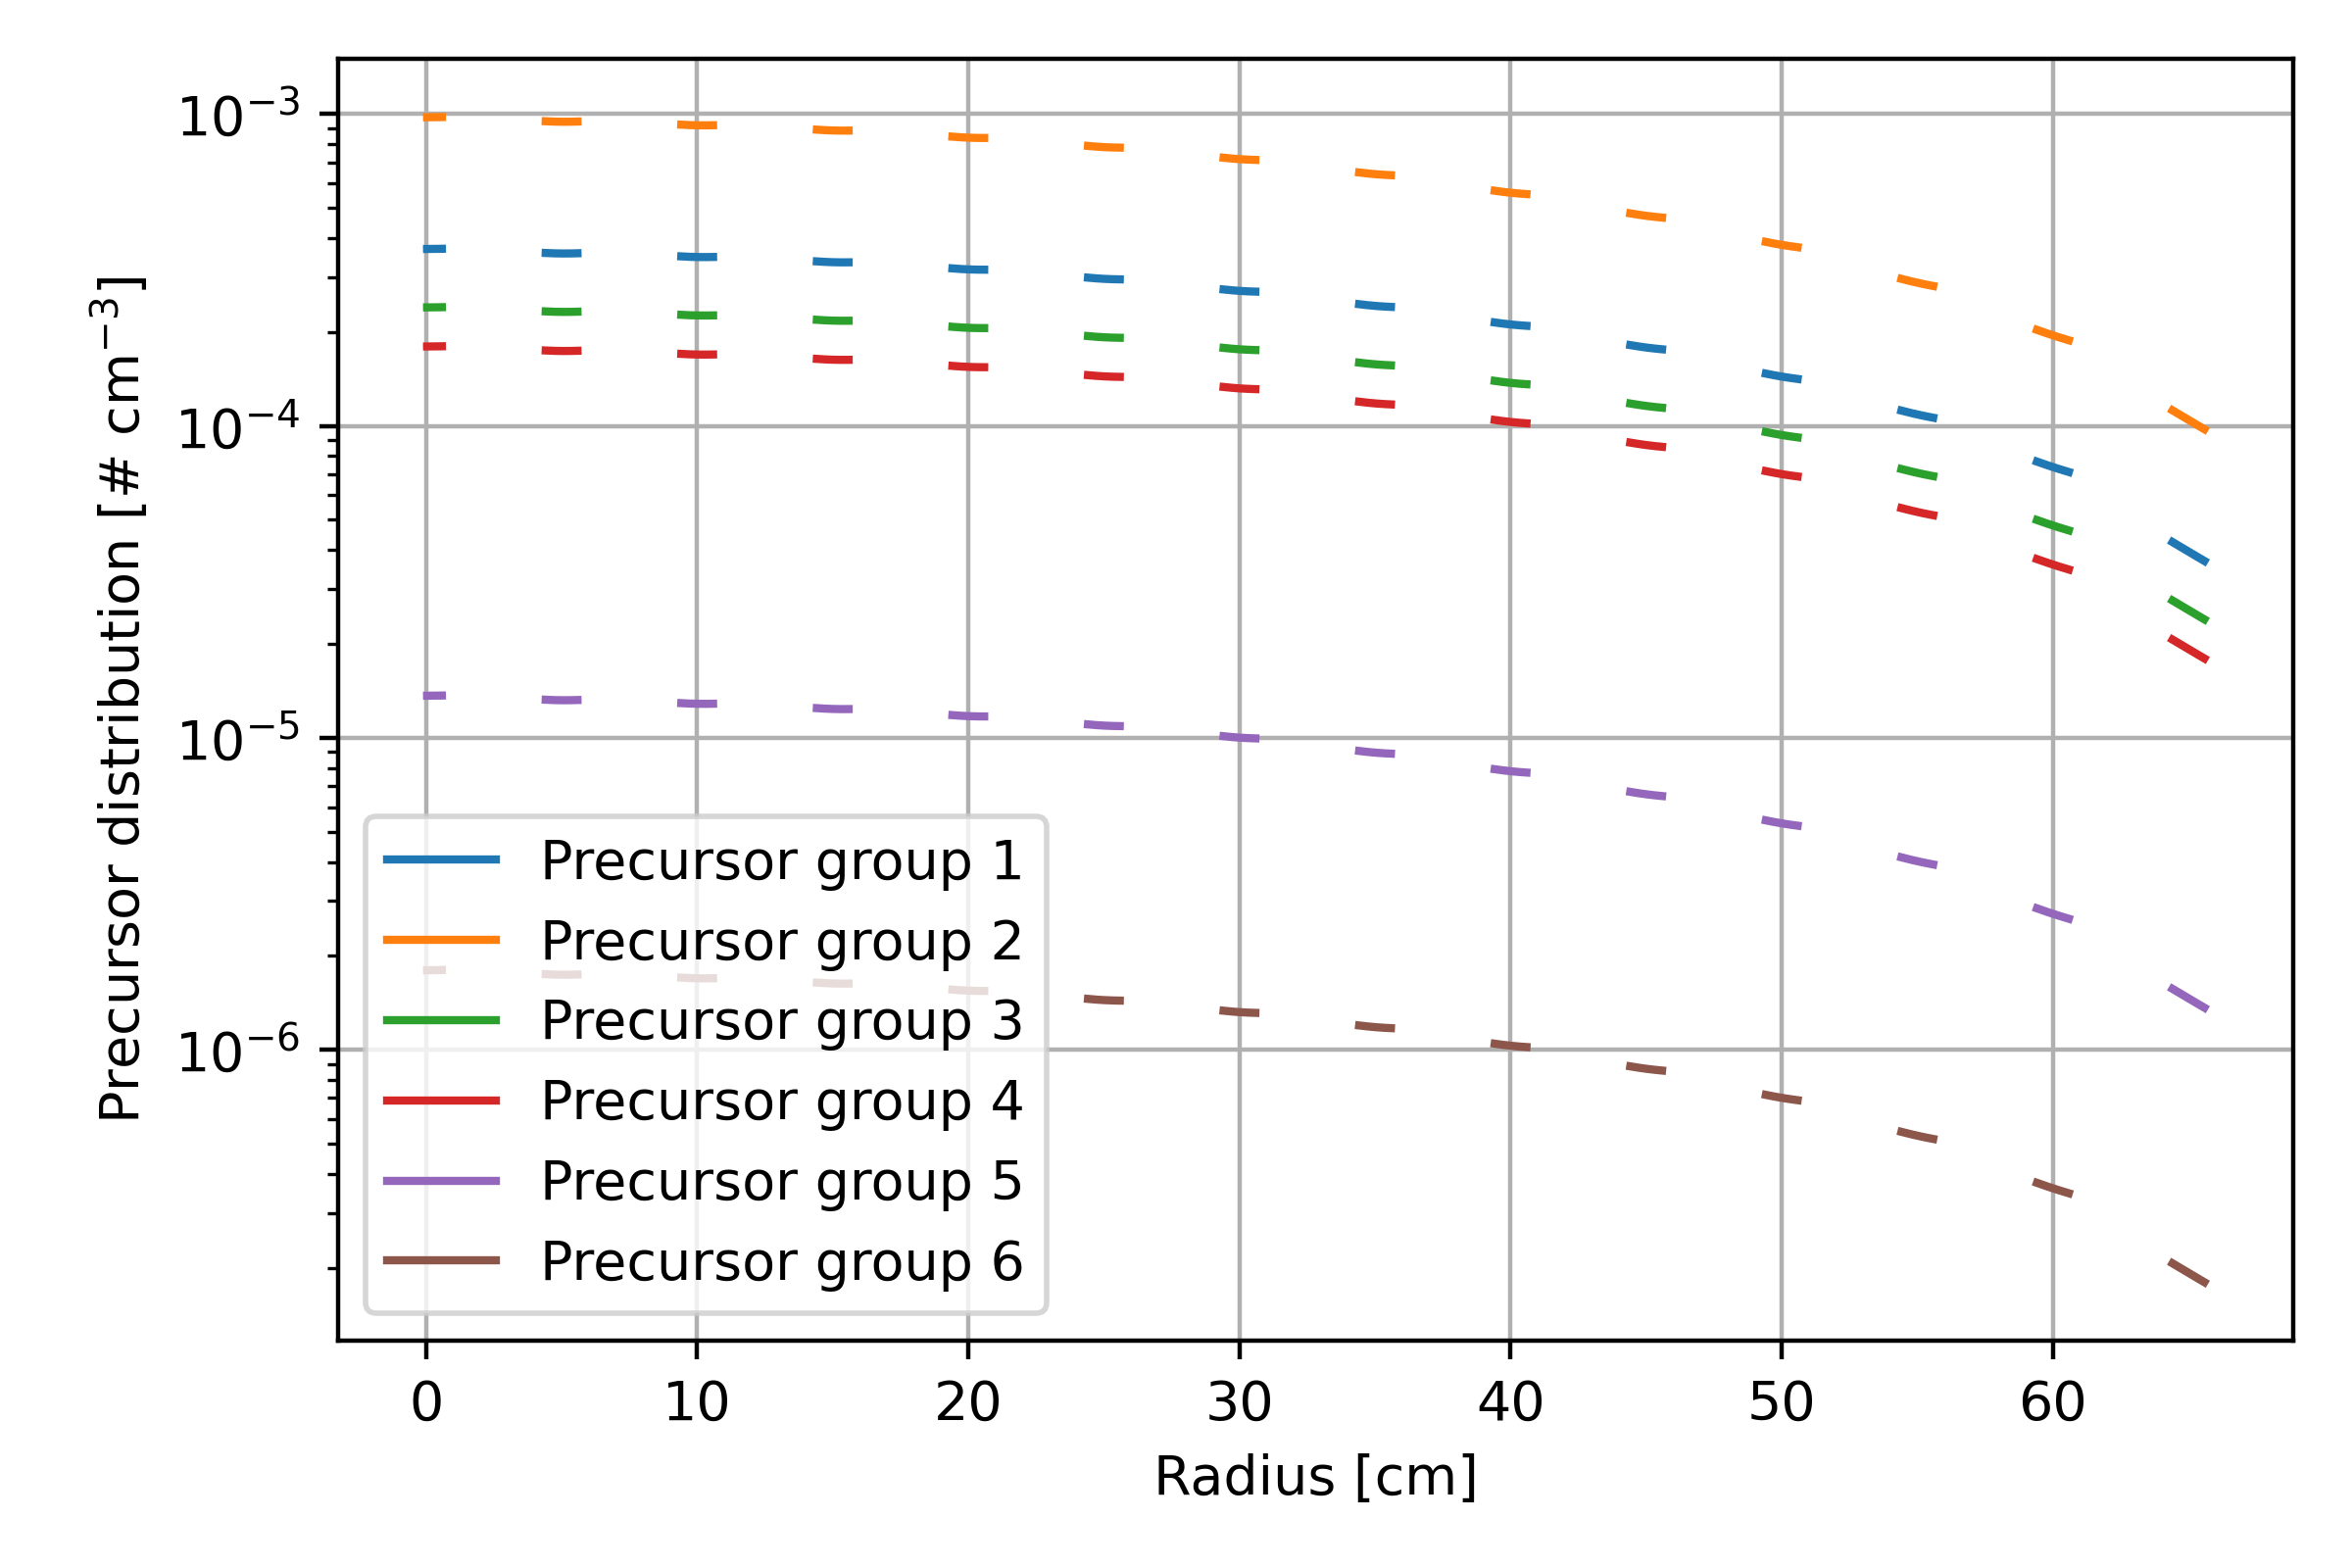
\includegraphics[width=\columnwidth]{midplane_pre}
    \caption{Normalized midplane \gls{DNP} distributions.}
    \label{fig:midplane-pre-dist}
  \end{subfigure}
  \hfill
  \begin{subfigure}[b]{0.48\columnwidth}
    \centering
    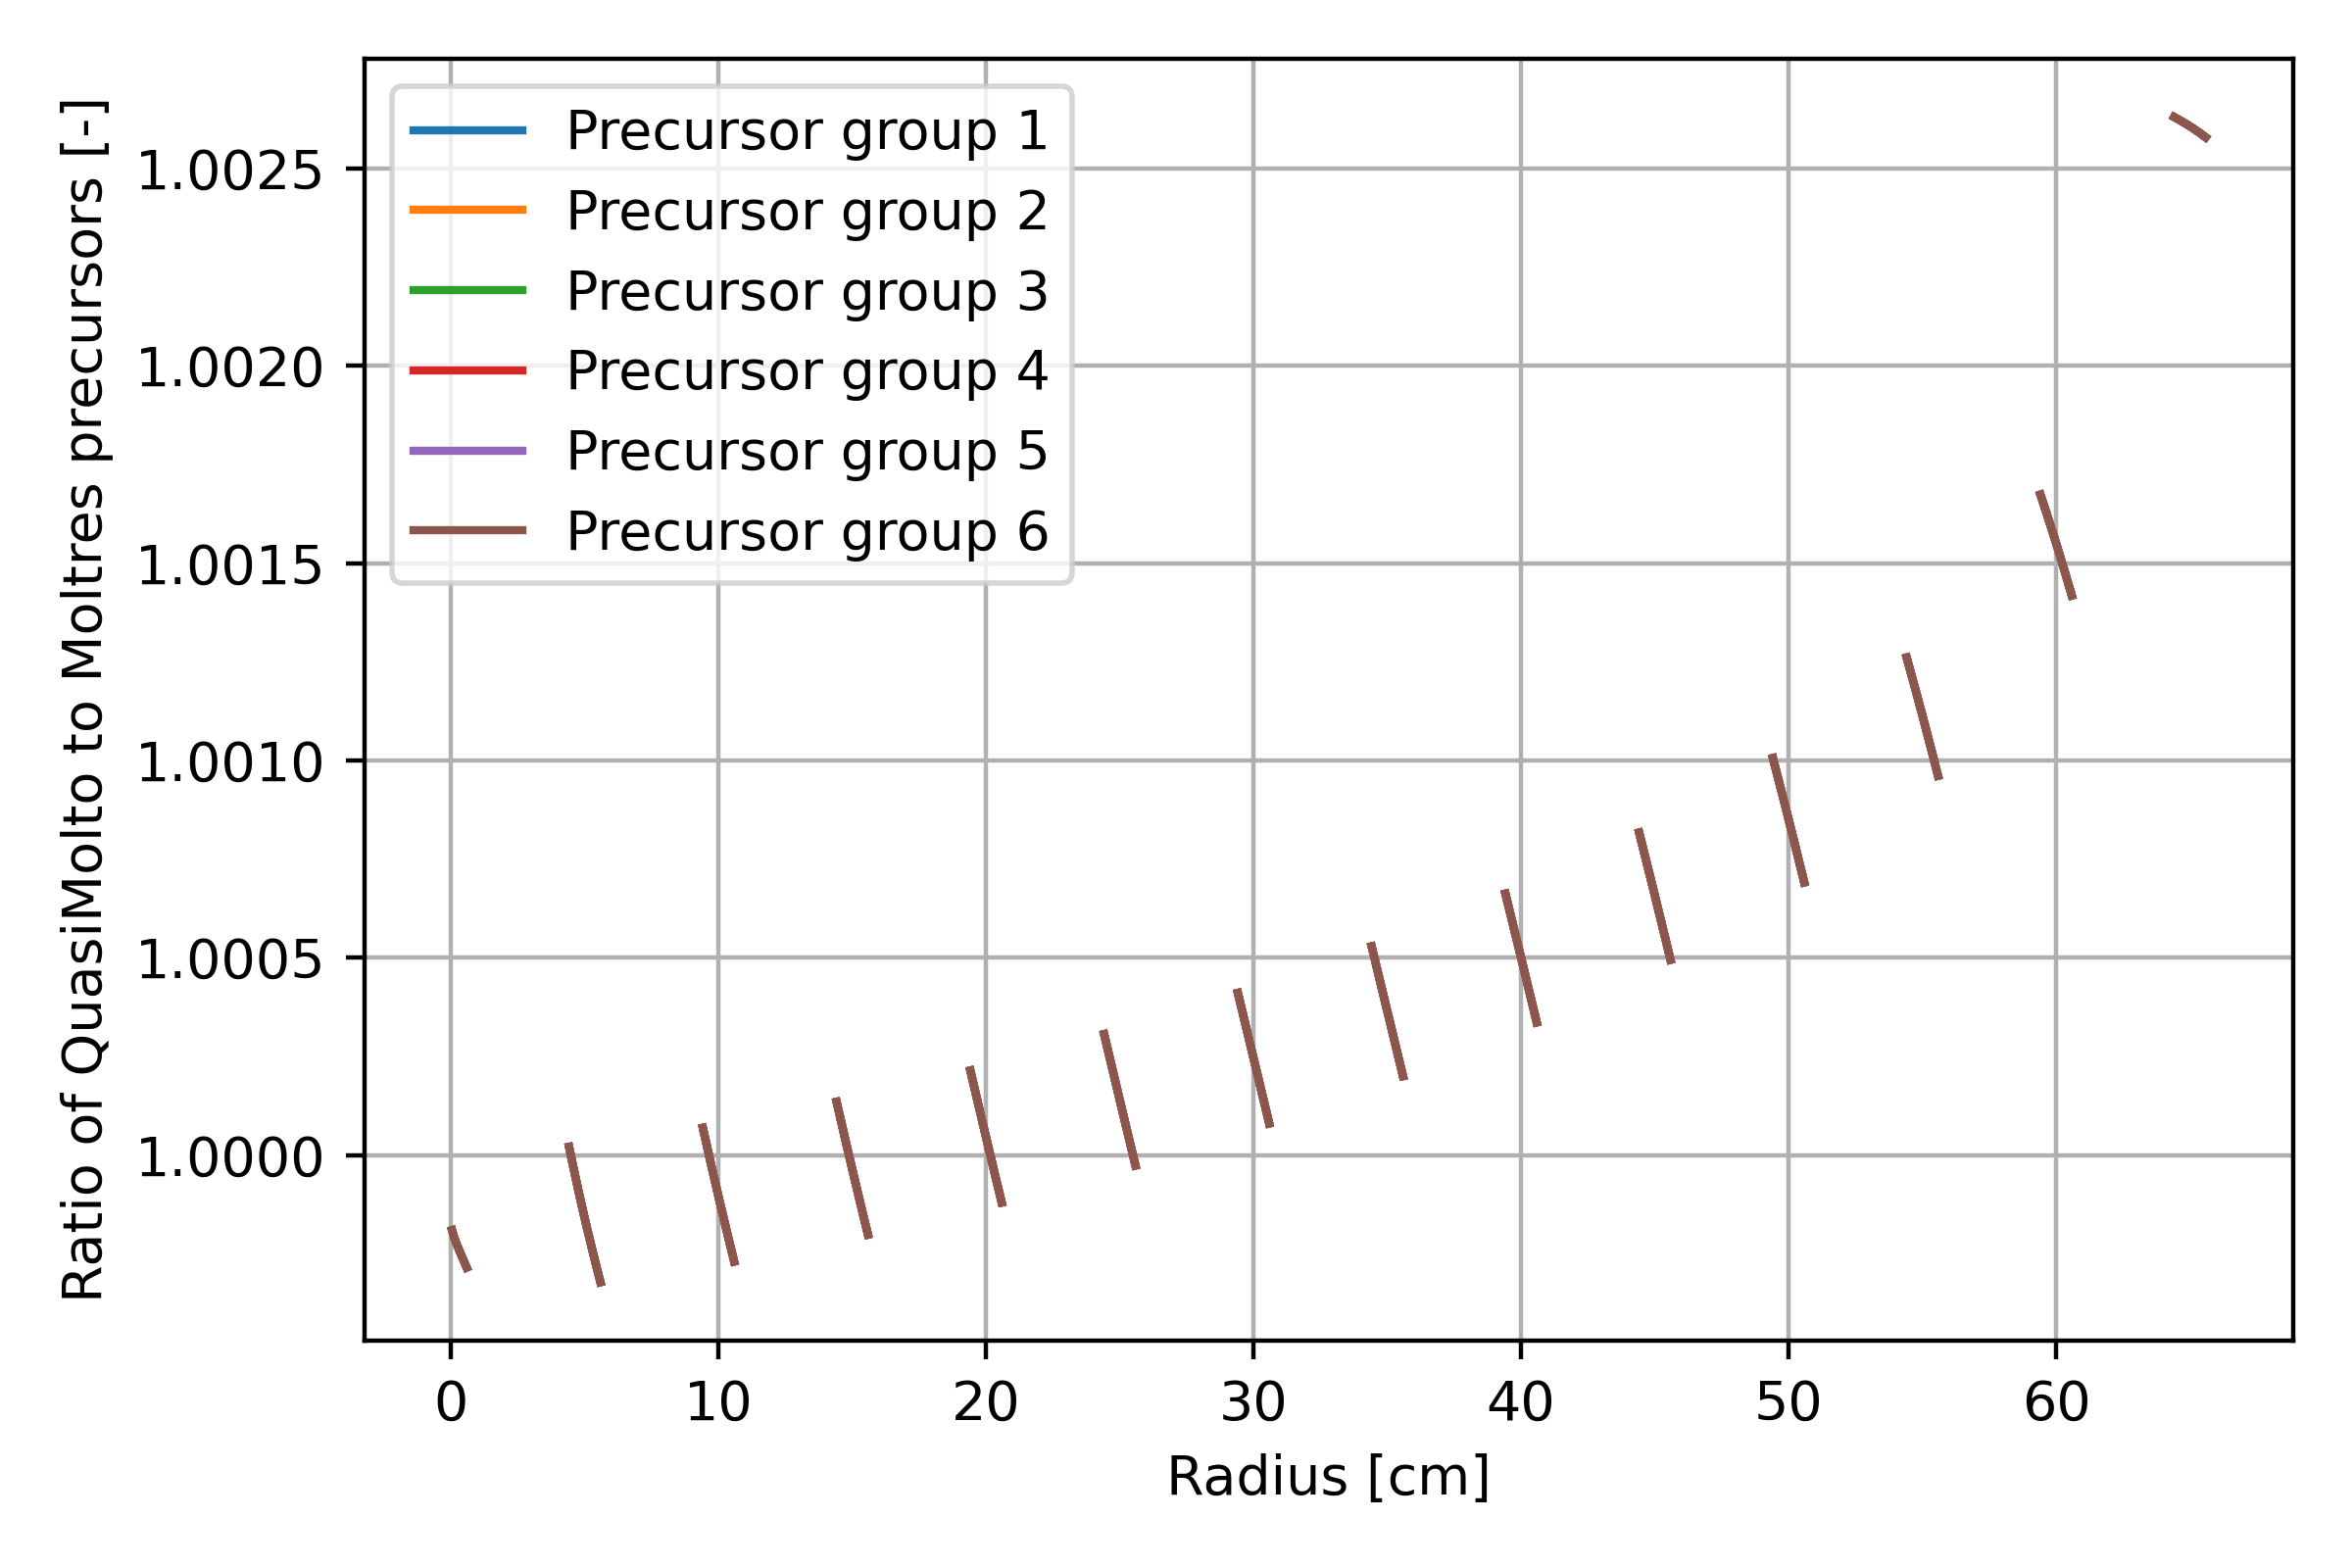
\includegraphics[width=\columnwidth]{midplane_pre_ratio}
    \caption{Ratio of midplane \gls{DNP} distributions.}
    \label{fig:midplane-pre-ratio}
  \end{subfigure}
  \caption{Midplane \gls{DNP} distribution from Moltres and ratios comparing QuasiMolto and Moltres
  models under static \gls{MSRE} conditions. \glspl{DNP} exist only in the fuel channel regions.
  The ratio curves for every \gls{DNP} group exhibit nearly perfect overlap.}
  \label{fig:midplane-pre}
\end{figure}

\begin{figure}[htb]
  \centering
  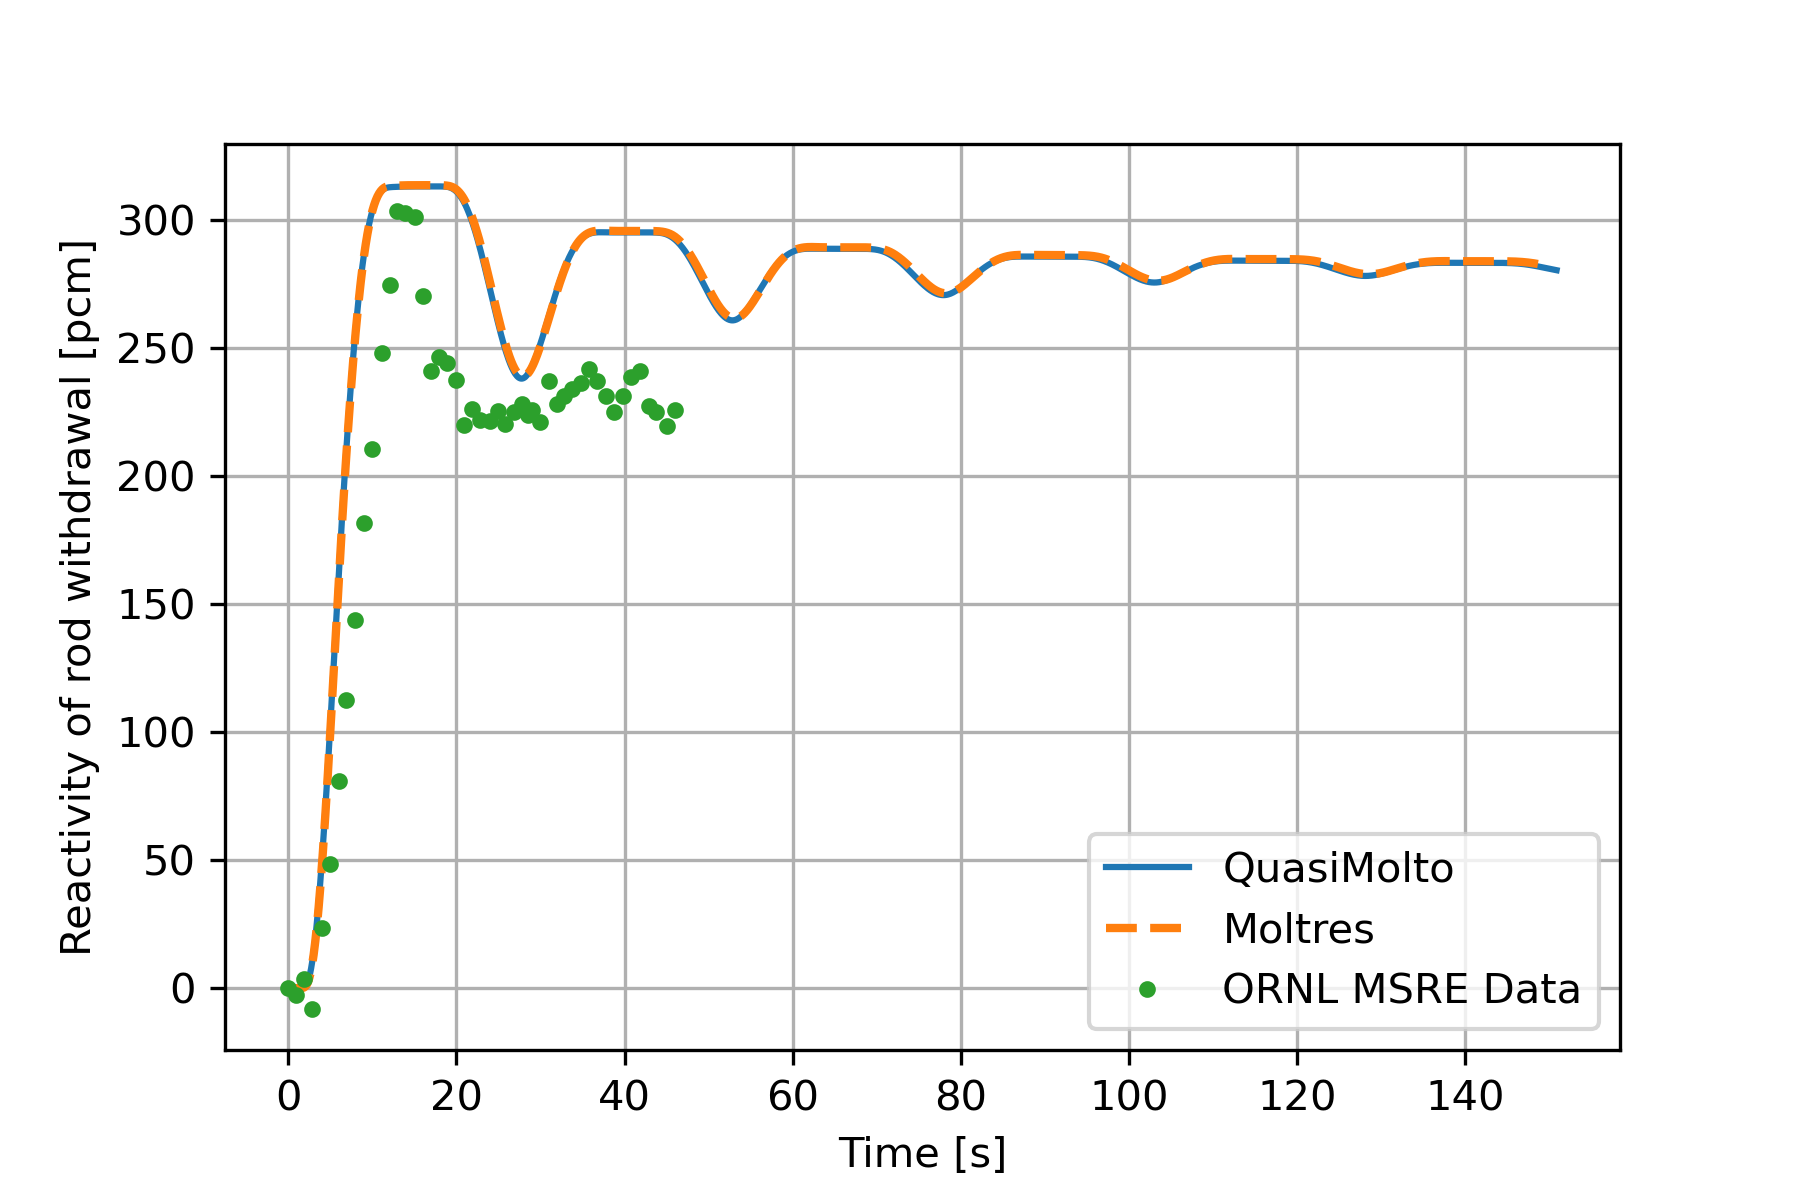
\includegraphics[width=0.9\columnwidth]{start-up-v2-reactivity}
  \caption{Reactivity (relative to static no-flow conditions) during the \gls{MSRE} pump start-up
  transient. The Moltres and QuasiMolto models agree closely with each other. The numerical models
  report greater peak and final reactivity change than the \gls{ORNL} \gls{MSRE} experimental
  data.}
  \label{fig:start-up-reactivity}
\end{figure}

\begin{figure}[htb]
  \centering
  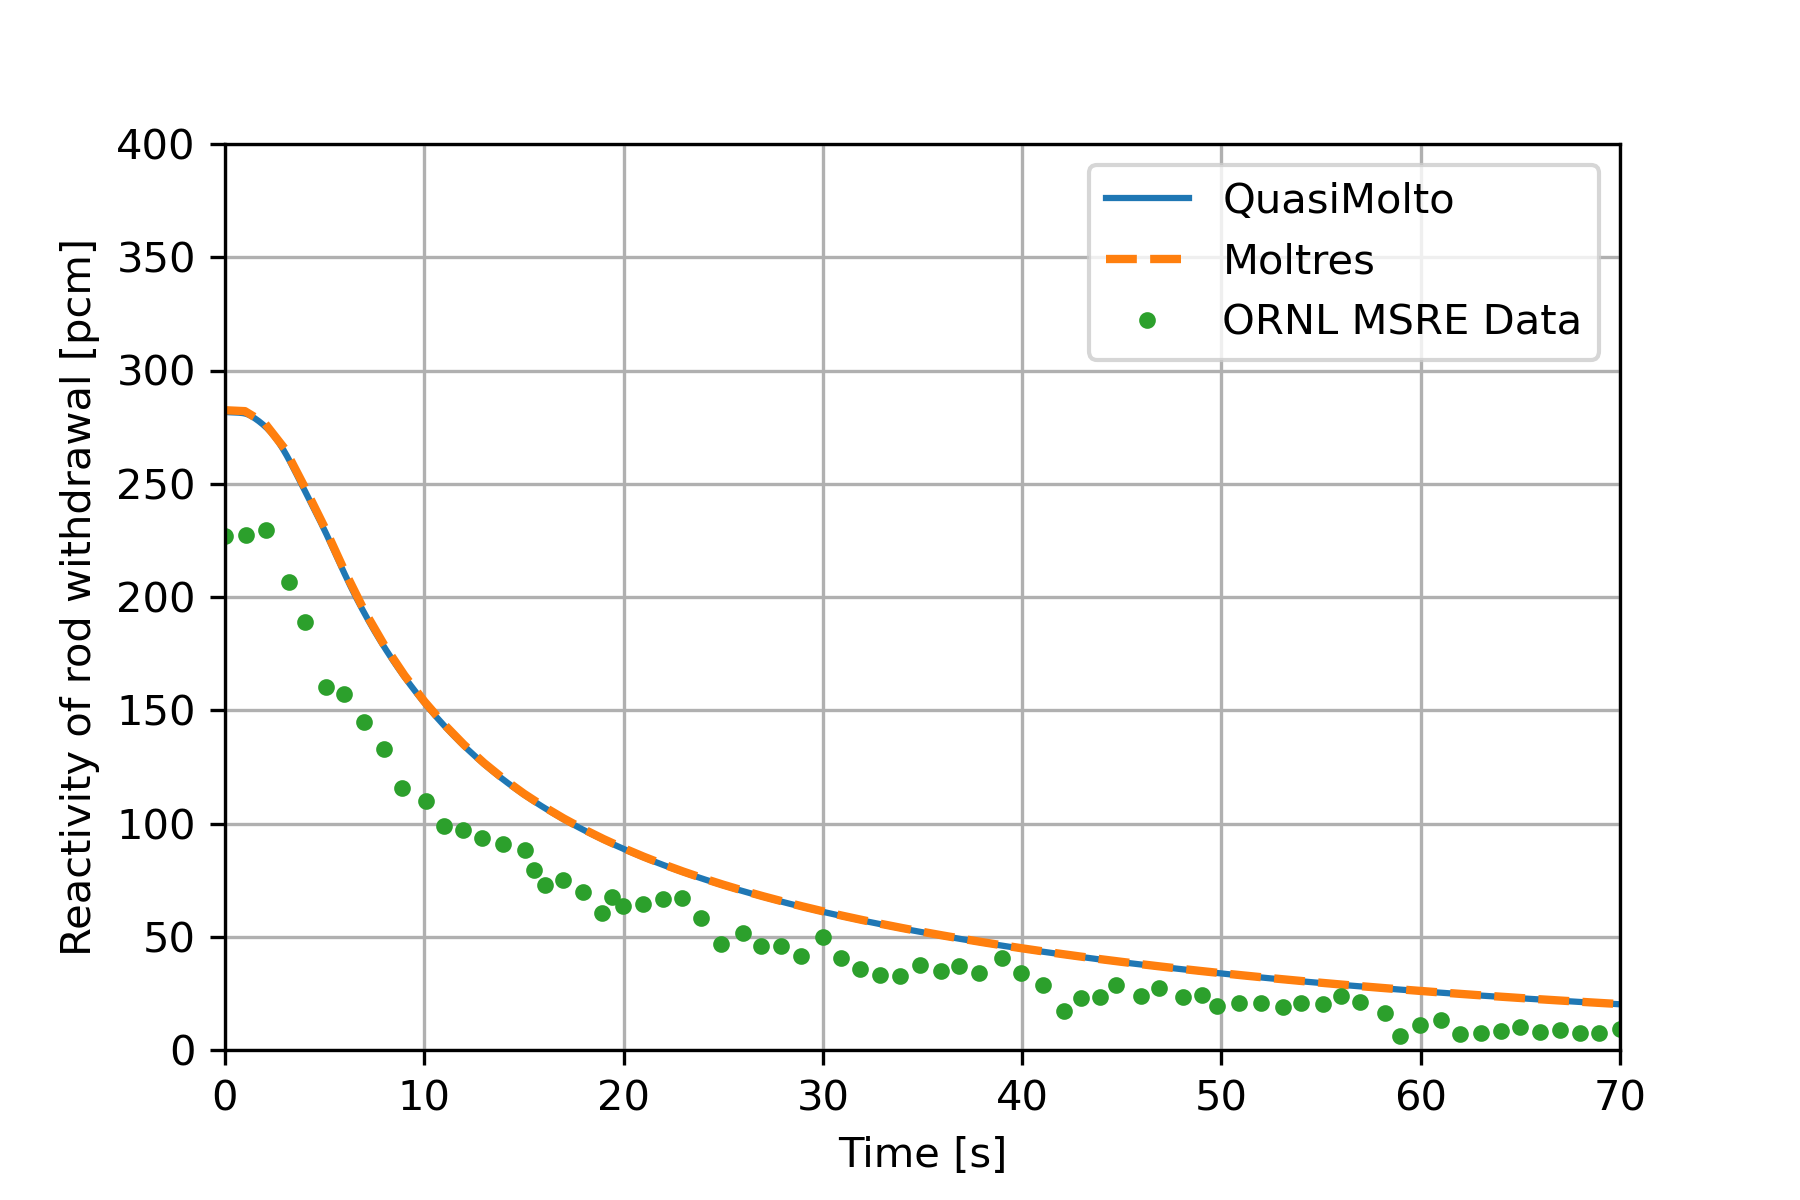
\includegraphics[width=0.9\columnwidth]{coast-down-v2-reactivity}
  \caption{Reactivity (relative to static no-flow conditions) during the \gls{MSRE} pump coast-down
  transient. The Moltres and QuasiMolto models agree closely with each other. The numerical models
  report greater reactivity change than the \gls{ORNL} \gls{MSRE} experimental data throughout the
  transient.}
  \label{fig:coast-down-reactivity}
\end{figure}

\subsection{Summary}

\FloatBarrier
